% This must be in the first 5 lines to tell arXiv to use pdfLaTeX, which is strongly recommended.
\pdfoutput=1
% In particular, the hyperref package requires pdfLaTeX in order to break URLs across lines.

\documentclass[11pt]{article}
\usepackage[utf8]{inputenc}
% \usepackage[latin1]{inputenc}

% Change "review" to "final" to generate the final (sometimes called camera-ready) version.
% Change to "preprint" to generate a non-anonymous version with page numbers.
\usepackage[final]{acl}
\usepackage{breakurl} 
% Standard package includes
\usepackage{times}
\usepackage{latexsym}
\usepackage{dsfont}
\usepackage{amsmath}
% For proper rendering and hyphenation of words containing Latin characters (including in bib files)
\usepackage[T1]{fontenc}
% For Vietnamese characters
% \usepackage[T5]{fontenc}
% See https://www.latex-project.org/help/documentation/encguide.pdf for other character sets

% This assumes your files are encoded as UTF8
\usepackage[utf8]{inputenc}

% This is not strictly necessary, and may be commented out,
% but it will improve the layout of the manuscript,
% and will typically save some space.
\usepackage{microtype}

% This is also not strictly necessary, and may be commented out.
% However, it will improve the aesthetics of text in
% the typewriter font.
\usepackage{inconsolata}
% \usepackage[numbers]{natbib}


%Including images in your LaTeX document requires adding
%additional package(s)
\usepackage{graphicx}
\usepackage{float}
\usepackage{multirow}
\usepackage{adjustbox}
\usepackage{booktabs}
\usepackage{amssymb}
\usepackage{amsmath}
\usepackage{subcaption}
\usepackage{xcolor}
\usepackage{fancyvrb}
\usepackage{lipsum}
\usepackage{listings}
\usepackage{xcolor}
\newtheorem{theorem}{Theorem}


\definecolor{green}{RGB}{0,100,0}


% If the title and author information does not fit in the area allocated, uncomment the following
%
%\setlength\titlebox{<dim>}
%
% and set <dim> to something 5cm or larger.

\title{Enrich-on-Graph: Query-Graph Alignment for Complex Reasoning with LLM Enriching}

% Author information can be set in various styles:
% For several authors from the same institution:
% \author{Author 1 \and ... \and Author n \\
%         Address line \\ ... \\ Address line}
% if the names do not fit well on one line use
%         Author 1 \\ {\bf Author 2} \\ ... \\ {\bf Author n} \\
% For authors from different institutions:
% \author{Author 1 \\ Address line \\  ... \\ Address line
%         \And  ... \And
%         Author n \\ Address line \\ ... \\ Address line}
% To start a separate ``row'' of authors use \AND, as in
% \author{Author 1 \\ Address line \\  ... \\ Address line
%         \AND
%         Author 2 \\ Address line \\ ... \\ Address line \And
%         Author 3 \\ Address line \\ ... \\ Address line}

\author{
    Songze Li\textsuperscript{1,3},
    Zhiqiang Liu\textsuperscript{1,3},
    Zhengke Gui\textsuperscript{2}, 
    Huajun Chen\textsuperscript{1,3},
    \textbf{Wen Zhang\textsuperscript{1,3}\thanks{~~Corresponding authors.}}\\
    \textsuperscript{1}Zhejiang University,
    \textsuperscript{2}Ant Group,
    \textsuperscript{3}ZJU-Ant Group Joint Lab of Knowledge Graph \\
    % $^\spadesuit$ Zhejiang University,
    % $^\diamondsuit$ Ant Group,
    % $^\clubsuit$ The University of Edinburgh\\
    % $^\heartsuit$ Zhejiang University - Ant Group Joint Laboratory of Knowledge Graph \\
    \texttt{
    \{li.songze,zhang.wen,huajunsir\}@zju.edu.cn
    }
}

%\author{
%  \textbf{First Author\textsuperscript{1}},
%  \textbf{Second Author\textsuperscript{1,2}},
%  \textbf{Third T. Author\textsuperscript{1}},
%  \textbf{Fourth Author\textsuperscript{1}},
%\\
%  \textbf{Fifth Author\textsuperscript{1,2}},
%  \textbf{Sixth Author\textsuperscript{1}},
%  \textbf{Seventh Author\textsuperscript{1}},
%  \textbf{Eighth Author \textsuperscript{1,2,3,4}},
%\\
%  \textbf{Ninth Author\textsuperscript{1}},
%  \textbf{Tenth Author\textsuperscript{1}},
%  \textbf{Eleventh E. Author\textsuperscript{1,2,3,4,5}},
%  \textbf{Twelfth Author\textsuperscript{1}},
%\\
%  \textbf{Thirteenth Author\textsuperscript{3}},
%  \textbf{Fourteenth F. Author\textsuperscript{2,4}},
%  \textbf{Fifteenth Author\textsuperscript{1}},
%  \textbf{Sixteenth Author\textsuperscript{1}},
%\\
%  \textbf{Seventeenth S. Author\textsuperscript{4,5}},
%  \textbf{Eighteenth Author\textsuperscript{3,4}},
%  \textbf{Nineteenth N. Author\textsuperscript{2,5}},
%  \textbf{Twentieth Author\textsuperscript{1}}
%\\
%\\
%  \textsuperscript{1}Affiliation 1,
%  \textsuperscript{2}Affiliation 2,
%  \textsuperscript{3}Affiliation 3,
%  \textsuperscript{4}Affiliation 4,
%  \textsuperscript{5}Affiliation 5
%\\
%  \small{
%    \textbf{Correspondence:} \href{mailto:email@domain}{email@domain}
%  }
%}

\begin{document}
\maketitle
\begin{abstract}
Large Language Models (LLMs) exhibit strong reasoning capabilities in complex tasks. However, they still struggle with hallucinations and factual errors in knowledge-intensive scenarios like knowledge graph question answering (KGQA). We attribute this to the semantic gap between structured knowledge graphs (KGs) and unstructured queries, caused by inherent differences in their focuses and structures. Existing methods usually employ resource-intensive, non-scalable workflows reasoning on vanilla KGs, but overlook this gap. To address this challenge, we propose a flexible framework, Enrich-on-Graph (EoG), which leverages LLMs' prior knowledge to enrich KGs, bridge the semantic gap between graphs and queries. EoG enables efficient evidence extraction from KGs for precise and robust reasoning, while ensuring low computational costs, scalability, and adaptability across different methods. Furthermore, we propose three graph quality evaluation metrics to analyze query-graph alignment in KGQA task, supported by theoretical validation of our optimization objectives. Extensive experiments on two KGQA benchmark datasets indicate that EoG can effectively generate high-quality KGs and achieve the state-of-the-art performance. Our code and data are available at \url{https://github.com/zjukg/Enrich-on-Graph}.
\end{abstract}

\section{Introduction}

\begin{figure}[h!]
    \centering
    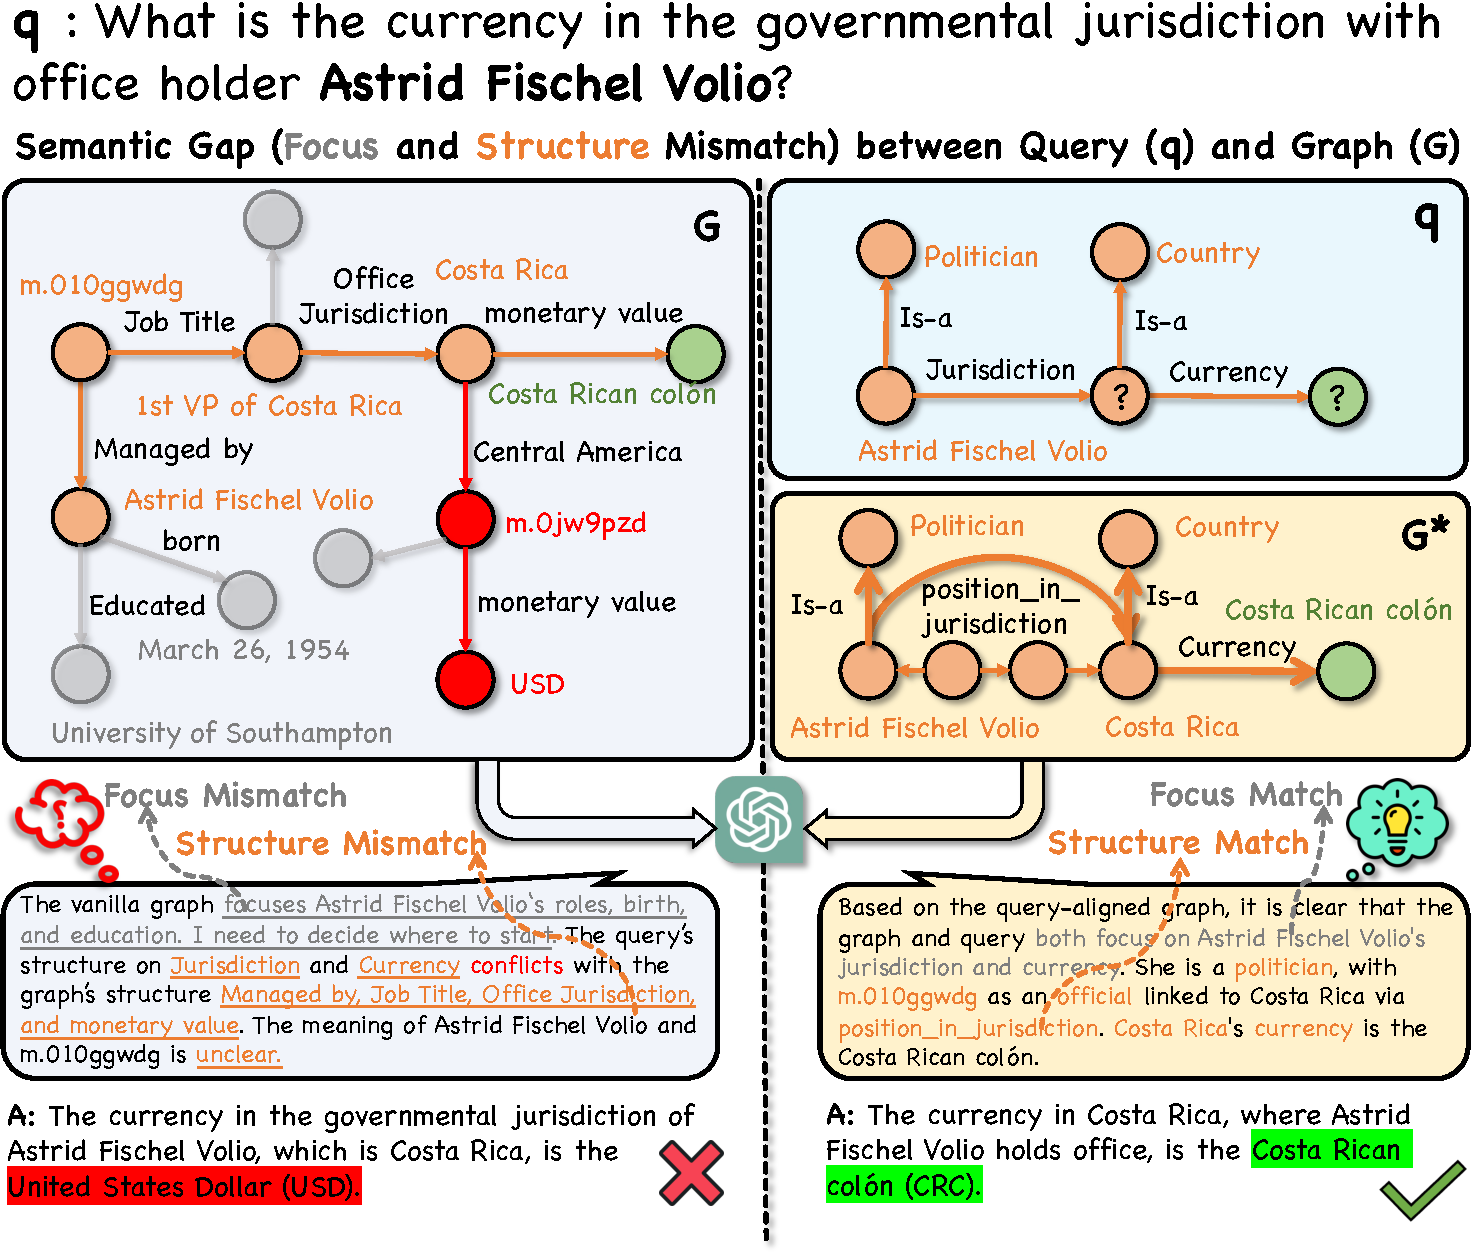
\includegraphics[width=\linewidth, keepaspectratio]{fig/intro3.pdf} 
    \caption{Semantic gap between query and graph: Gray indicates noise, red represents errors, orange denotes reasoning-related information, and green is answer. We use $ G $, $ Q $, $ G^* $ to represent vanilla graph, query, query-aligned graph, respectively, and use their logic forms for illustration.
\textbf{Left:} LLMs misextracts key information due to the semantic gap between \(Q\) and \(G\).
\textbf{Right:} EoG generates \(G^*\) for efficient LLM reasoning.}
    \label{fig:intro1}
\end{figure}

% Large language models (LLMs) have exhibited strong capabilities across various natural language processing tasks, particularly in complex reasoning scenarios. Through extensive pre-training on large corpora, these models have acquired substantial prior knowledge encoded within their parameters, which is beneficial for reasoning and semantic understanding in complex tasks. This prior supports LLMs in handling complex reasoning and generating informed responses to challenging queries, making them effective in diverse question-answering tasks. However, LLMs still encounter issues such as hallucinations and outdated knowledge, especially in knowledge-intensive scenarios. As shown in Fig.~\ref{fig:intro1}, the lack of specific knowledge about \textit{Astrid Fischel Volio} leads to difficulties in producing accurate responses, ultimately undermining the dependability of LLMs.


Large language models (LLMs)~\cite{openai2024gpt4technicalreport,brown2020languagemodelsfewshotlearners,chowdhery2022palmscalinglanguagemodeling,azaria2024chat} excel in complex natural language processing (NLP) tasks~\cite{wei2023chainofthoughtpromptingelicitsreasoning,khot2023decomposedpromptingmodularapproach,li2023evaluation} due to extensive pre-training on large corpora~\cite{rawte2023surveyhallucinationlargefoundation} embedding prior knowledge in their parameters~\cite{khot2023decomposedpromptingmodularapproach}.
% Large language models (LLMs)~\cite{openai2024gpt4technicalreport,brown2020languagemodelsfewshotlearners,chowdhery2022palmscalinglanguagemodeling} excel in natural language processing (NLP), especially in complex reasoning tasks~\cite{wei2023chainofthoughtpromptingelicitsreasoning,khot2023decomposedpromptingmodularapproach}, due to extensive pre-training on large corpora~\cite{rawte2023surveyhallucinationlargefoundation} that embeds prior knowledge in their parameters~\cite{khot2023decomposedpromptingmodularapproach}. 
Based on the prior knowledge, LLMs can achieve semantic understanding, perform reasoning, and generate reasonable responses in diverse question-answering tasks~\cite{li2023unigenunifiedgenerativeframework,zhao2024generating}. However, LLMs still face challenges like hallucinations and factual errors~\cite{Ji_2023,chen2024large}, particularly in knowledge-intensive scenarios like knowledge graph question answering. 
% For instance, as shown in Fig.~\ref{fig:intro1}(a), lacking specific knowledge about \textit{Astrid Fischel Volio} impacts response accuracy, reducing reliability.

Knowledge graph question answering (KGQA) is the task of answering natural language queries based on structured factual information stored in knowledge graphs (KGs)~\cite{DBLP:conf/semweb/AuerBKLCI07,freebase}. Existing KGQA methods can be broadly categorized into information retrieval-based and semantic parsing-based.
Information retrieval~\cite{sun-etal-2019-pullnet,zhang-etal-2022-subgraph} methods extract subgraphs relevant to a query and reason over them, but retrieval process inevitably introduces noise, thereby reducing accuracy of answer. Semantic parsing methods~\cite{sun2020sparqaskeletonbasedsemanticparsing,jiang2023unikgqa} generate logical forms (e.g., SPARQL) for querying KGs. 
However, both approaches remain limited by the reasoning capabilities of their underlying models, especially for complex queries.

Given LLMs' strong understanding and reasoning capabilities, advanced methods usually employ LLMs for KGQA. 
\textit{We believe that the core of such methods lies in how to bridge the \textbf{Semantic Gap Between Queries and Knowledge Graphs}}, which stems from the focus and structure mismatch. User query is a precise, goal-driven request with clear semantic focus. In contrast, KGs encompass diverse focuses across many topics, often containing substantial noisy information. This focus mismatches between the query and the KG makes it challenging to accurately retrieve the subgraphs needed for reasoning. Even when relevant subgraphs are retrieved, the rigid structure of KGs often clashes with the linguistic diversity of user queries, complicating reasoning.
As shown in Fig.~\ref{fig:intro1} Left, the vanilla graph contains significant noise (gray entities), which is mismatched with the query focus. The query, \textit{``What is the currency in the governmental jurisdiction with office holder Astrid Fischel Volio?"}, requires a two-hop reasoning path (\textit{Jurisdiction → Currency}), but the vanilla graph uses a 4-hop path (\textit{Managed → Job → Office Jurisdiction → Monetary Value}) and involves ambiguous entity \textit{Astrid Fischel Volio}, creating a structure mismatch.
% Consequently, the performance of existing methods suffers from focus and structure mismatches when relying on reasoning over vanilla KGs.
Consequently, reasoning over vanilla KGs is hindered by focus and structure mismatches. 

% Given LLMs' strong understanding and reasoning capabilities, 
% advanced KGQA methods usually employ LLMs for intricate reasoning pipelines to enhance performance, which demands substantial computational resources and operational costs.
\textbf{Previous methods struggle to align the semantics between queries and graphs from the perspective of designing complex reasoning pipelines}, which can be effective at times but come with high computational or training costs that hinder their efficiency.
% while their performance is limited by the semantic gap between queries and vanilla graphs.
For example, the DoG~\cite{ma2025debate} framework iteratively simplifies queries and focuses on subgraphs through steps like Invoking, Filtering, Answer Trying, and Simplifying, enabling step-by-step reasoning but leading to a rigid and bulky workflow. RoG~\cite{luo2024reasoninggraphsfaithfulinterpretable} requires fine-tuning LLMs for relationship path planning, which extracts query-relevant subgraph relations for faithful reasoning, but making adaptation to different KGs costly due to retraining. ToG~\cite{sun2023thinkongraph} leverages LLMs to explore and reason over entities and relations in KG based on the query in an iterative manner. 
These methods attempt to align the semantics between queries and graphs through reasoning, but they still suffer from the semantic gap when reasoning over vanilla KGs.
% However, the performance of existing methods suffers from focus and structure mismatches when relying on reasoning over vanilla KGs.
% We find that previous methods often rely on LLMs to interact with graph evidence based on the semantics of query to facilitate reasoning. 


To address the challenge, we propose Enrich-on-Graph (EoG), a flexible three-stage framework that leverages LLMs' prior knowledge to enrich graph, aligning the semantics between the vanilla KGs and queries. 
EoG proceeds in three stages: 
(1) \textbf{Parsing:} parsing the query and graph to enable effective alignment;
(2) \textbf{Pruning:} proposing focus-aware multi-channel pruning to mitigate focus mismatches;
(3) \textbf{Enriching:} leveraging LLMs to enrich graph to resolve structure mismatches.
The aligned graph then collaborates with LLMs as an external knowledge source for efficient reasoning, shown in Fig.~\ref{fig:intro1} Right. 
We also introduce three graph quality metrics—\textbf{Relevance, Semantic Richness}, and \textbf{Redundancy}—to evaluate graphs' structural properties, feature attributes, and LLM-driven aspects, supported by theoretical analyses further linking these metrics to optimization objectives.
The major contributions of this work are as follows:

\begin{itemize}
\item We highlight the key of KGQA task lies in how to bridge the semantic gap between queries and KGs. We further propose three graph quality metrics—Relevance, Semantic Richness, and Redundancy. Theoretical analyses validate alignment mechanism's effectiveness and the practical utility of these metrics.

\item We propose a flexible Enrich-on-Graph (EoG) framework that leverages LLMs as prior to align the semantics between queries and graphs, enabling high-quality KG generation and precise reasoning.

\item Extensive experiments on two KGQA benchmark datasets demonstrate that EoG achieves the state-of-the-art performance through generating high-quality KGs, while ensuring flexibility, low computational cost, scalability, and broad compatibility with other methods.
\end{itemize}

\section{Task Formulation and Analysis}
\label{sec:methods}
\subsection{Task Formulation}
% Given a KG, which stores a large amount of factual knowledge in the form of triples.
% \[G = \left\{ \left( {e_{s},r,e_{o}} \right) \middle| e_{s},e_{o}\in E,r\in R \right\},\]
% where \(E\) is the set of entities, and \(R\) is the set of relations.
% In complex KGQA tasks, given a complex user query \(q\) (e.g., \textit{What is the currency in the governmental jurisdiction with office holder Astrid Fischel Volio?}), the query can be hierarchically decomposed into several sub-queries, such as \(q_1\) (\textit{Who is Astrid Fischel Volio?}) and \(q_2\) (\textit{What areas does Astrid Fischel Volio govern or oversee?}), collectively forming a set of query \(Q\).
% \[Q = \left\{ q,q_{1},q_{2},q_{3},\ldots,q_{k} \right\}\]
% We define $  G^*  $ as the graph that is aligned with query. 
% By using $  G  $ as the external knowledge source to assist the prediction model, LLM $  M_{\theta}  $, in completing the QA task, our goal is:
% \[a^{*} = M_{\theta}\left( {Q,G} \right),\]
% where $  a^*  $ is the correct answer to the query $  q  $.

Given a KG $G = \left\{ \left( {e_{s},r,e_{o}} \right) \middle| e_{s},e_{o}\in E,r\in R \right\}$, where $E$ and $R$ are the set of entities and relations, it stores a large amount of factual knowledge in the form of triples. For a complex query $q$, the goal of the KGQA method $M_{\theta}$ with parameters $\theta$ is to get the correct answer $a^*$ that $a^* = M_{\theta}(q, G)$. 

\subsection{Semantic Gap between Query and Graph}
\label{Semantic Gap between Query and Graph}

\begin{figure}[h!]
    \centering
    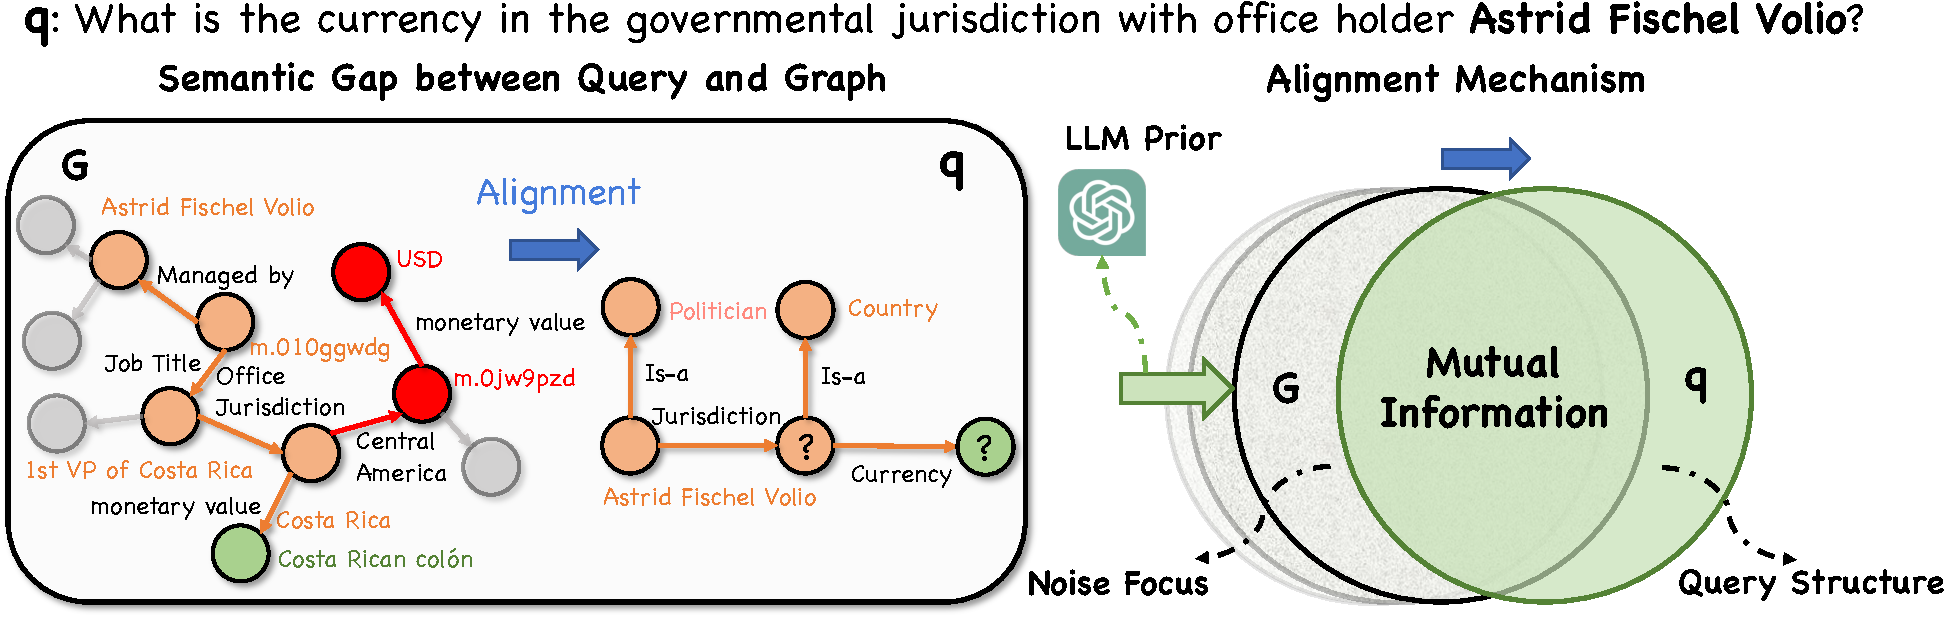
\includegraphics[width=\linewidth, keepaspectratio]{fig/method1.pdf}
    \caption{\textbf{Left:} focus mismatch and structure mismatch between query and vanilla graph cause semantic gaps.
\textbf{Right:} Demonstration of EoG's alignment mechanism.}
    \label{fig:method1}
\end{figure}

To better illustrate that the semantic gap between the KG and the query arises from \textbf{focus mismatch} and \textbf{structure mismatch}, we refer to previous works~\cite{wang2023knowledgedrivencotexploringfaithful,DBLP:conf/aaai/ZhangZMWS0SZ24} to visualize their logical forms, as shown in Fig.~\ref{fig:method1} (left).
\paragraph{Focus Mismatch:} For the query \textit{``What is the currency in the governmental jurisdiction with office holder Astrid Fischel Volio?"}, it explicitly focuses on the jurisdiction managed by \textit{Astrid Fischel Volio} and its currency, represented as: \textit{Astrid Fischel Volio → Jurisdiction → ? → Currency → ?}. However, the vanilla KG includes irrelevant focuses, such as \textit{Astrid Fischel Volio}’s birthday and education (gray nodes), which we call focus mismatch since they do not help the reasoning process.
\paragraph{Structure Mismatch:} As shown in Fig.~\ref{fig:method1} (left), the vanilla KG contains 4-hop structures (orange nodes): \textit{Astrid Fischel Volio → Managed → m.010ggwdg → Job → 1st VP of Costa Rica → Office Jurisdiction → Costa Rica → Monetary Value → Costa Rican colón}. In contrast, the query has corresponding 2-hop structures: \textit{Jurisdiction → Currency}. The \textbf{structure inconsistency in reasoning hops} (e.g., the query’s single-hop \textit{Jurisdiction} versus KG’s 3-hop \textit{Managed → Job → Office Jurisdiction}) makes multi-hop reasoning harder for LLMs. Additionally, ambiguous entities like \textit{Astrid Fischel Volio} (\textbf{lacking a hierarchy structure} such as \textit{Astrid Fischel Volio → is-a → Politician}) further confuse LLMs. These issues are referred to as structure mismatch.
In summary, \textbf{the semantic gap between the vanilla KG and the query} stems from \textbf{focus mismatch} and \textbf{structure mismatch}.

\section{Method}
\subsection{Solution of EoG}
As shown in Fig.~\ref{fig:method1} (left), ideally, for complex KGQA tasks, we want to use a graph $G^*$ that is consistent with the logic form of $q$ to help LLMs reason efficiently. However, in reality, we can only use the vanilla KG $G$, letting LLMs leverage external knowledge from $G$ and its pre-trained knowledge to find information relevant to $q$ for answering. Thus, our goal is to find an optimized graph $G^*$ by maximizing the expected posterior probability:

% For complex KGQA tasks, our goal is that given $G$, the LLM leverages external knowledge from $G$ and its pre-trained parametric knowledge to identify information relevant to $Q$, enabling efficient question answering. Therefore, we aim to find an optimized graph $G^*$ by maximizing the expected posterior probability:
\[{G^{*} = \underset{G}{argmax}}{~\mathbb{E}_{P(q,G)}\left\lbrack P\left( M_{\theta},q \middle| G \right) \right\rbrack}\]
By identifying the optimized graph $  G^*  $, the LLM $  M_{\theta}  $ can directly extract key knowledge from $  G^*  $ to better perform reasoning on $q$ and arrive at $a^*$.
\begin{theorem}
Maximizing the expected posterior probability is equivalent to maximizing the mutual information (MI) between $q$ and $G$.
\end{theorem}
\label{theorem1}
% \textbf{Theorem1:} Maximizing the expected posterior probability is equivalent to maximizing the mutual information between Q and G.

{\small
\[P\left( M_{\theta},q \middle| G \right) \propto {\log\left( \frac{P\left( M_{\theta},q \middle| G \right)}{P(q)} \right)}{{= \log}\left( \frac{P\left( M_{\theta},G \middle| q \right)}{P(G)} \right)}\]
}
{\small
\[\propto {\log\left( \frac{\int_{M_{\theta}}^{}{P\left( M_{\theta},G \middle| q \right)dM_{\theta}}}{P(G)} \right)} = {\log\left( \frac{P\left( {q,G} \right)}{P(q)P(G)} \right)}\]
}
Therefore, we can obtain (Details in Appendix~\ref{Details of our Theoretical Proof}):
\[\mathbb{E}_{P(q,G)}\left\lbrack {P\left( M_{\theta},q \middle| G \right)} \right\rbrack \propto MI(q,G)\]

As shown in Fig.~\ref{fig:method1} (right), through maximizing $MI(q, G)$, $G$ eliminates focus mismatch and structure mismatch, resulting in the desired $G^*$.

\subsection{Our Method: Enrich-on-Graph (EoG)}
\begin{figure*}[ht]
    \centering
    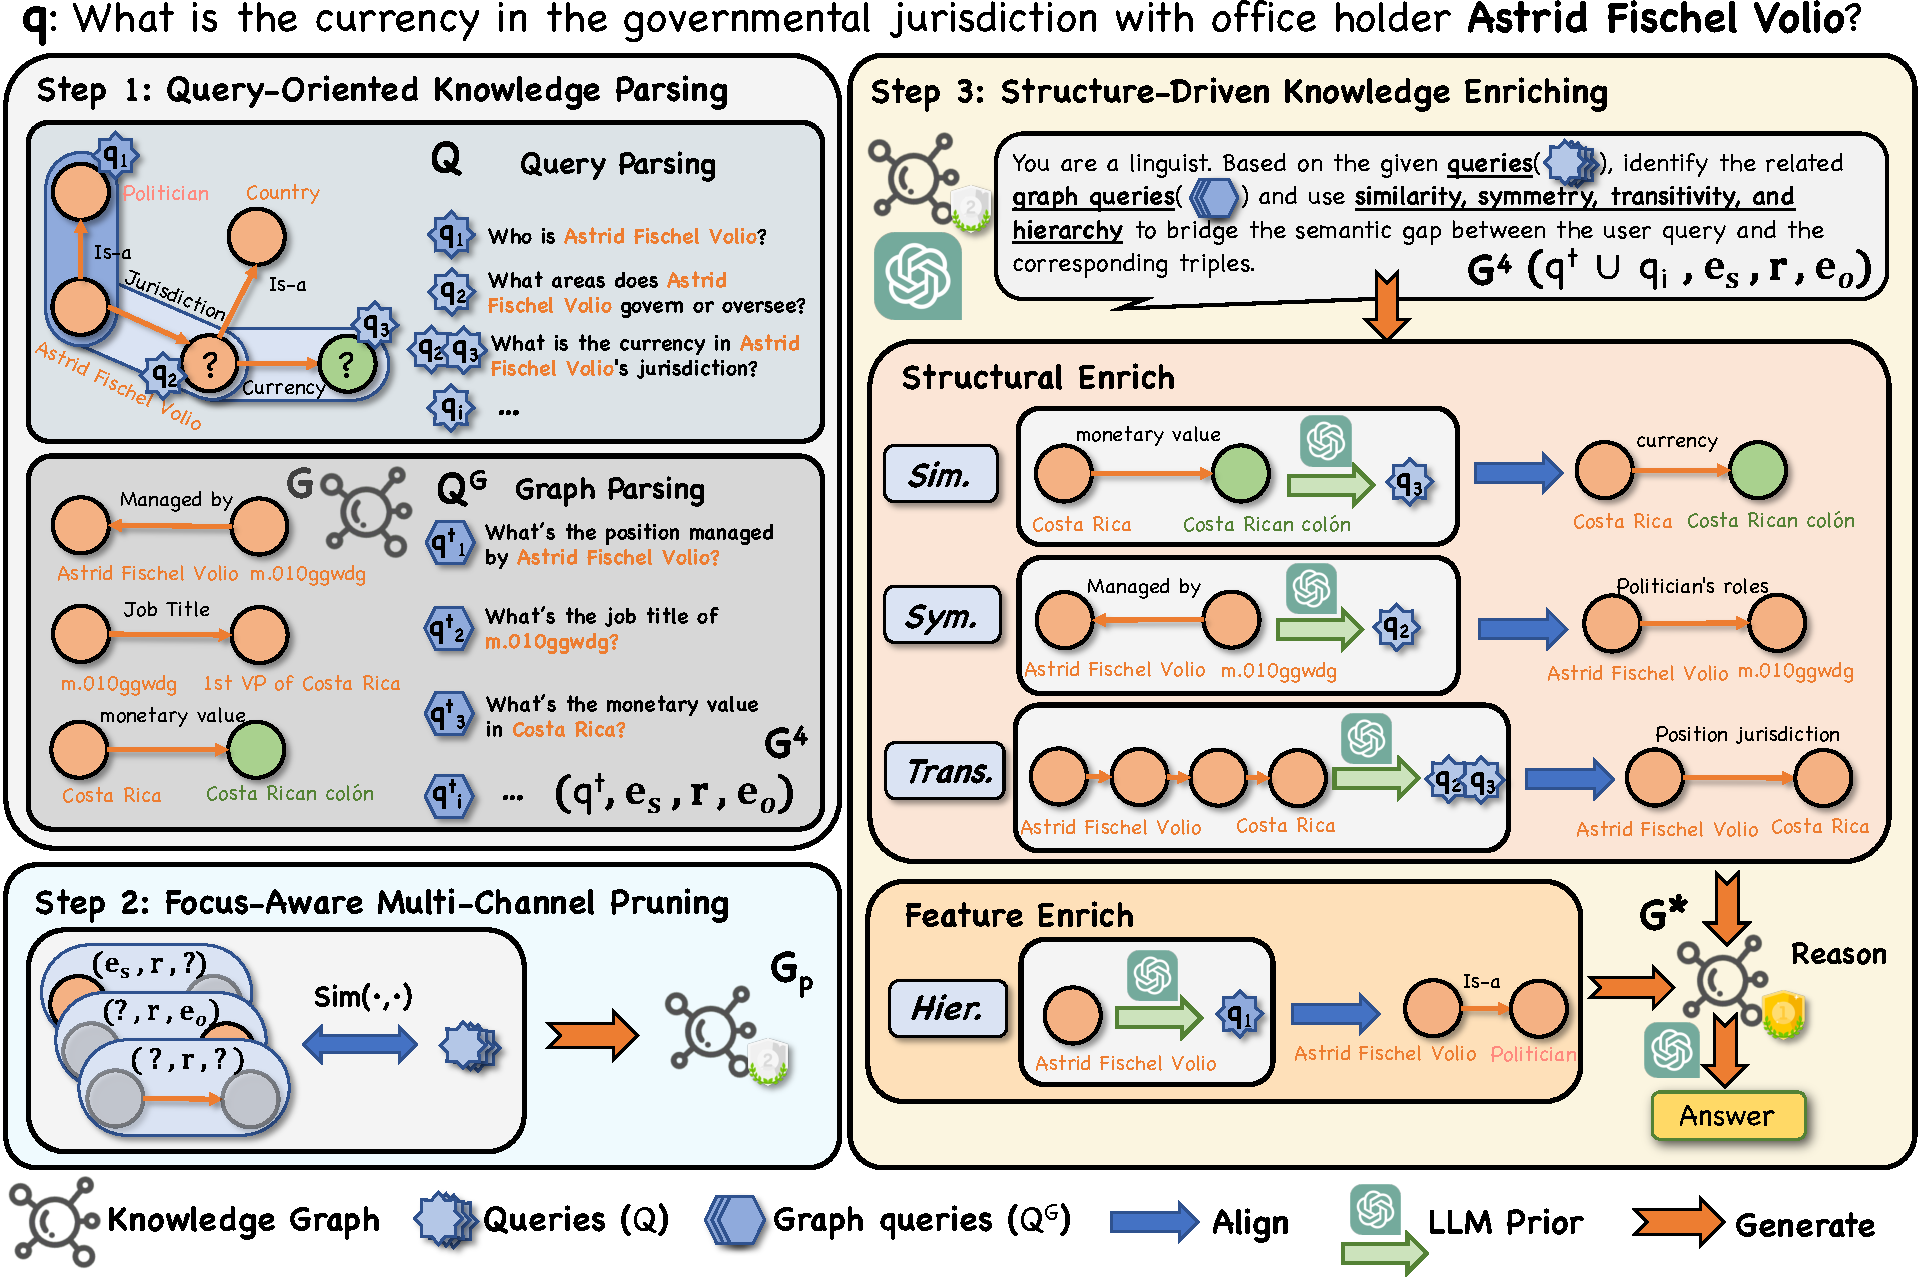
\includegraphics[width=1.0\textwidth, keepaspectratio]{fig/method2.pdf}
    \caption{Overview of our Enrich-on-Graph framework.}
    \vspace{-4mm}
    \label{fig:method2}
\end{figure*}

As shown in Fig.~\ref{fig:method2}, given a user query $q$ and a vanilla graph $G$, our method consists of three stages:
\textbf{(1) Parsing:} we parse $q$ into new forms $Q$, while converting $G$ into a query form $Q^G$ (which we refer to as the graph query) and injecting it into triples to construct quadruples, preparing for the better semantic alignment.
\textbf{(2) Pruning:} Using the $Q$ from the first stage, we prune noisy graph focuses via multiple channels, eliminating focus mismatches.
\textbf{(3) Enriching:} Leveraging LLMs with parametric knowledge as prior, $Q^G$ related to the $Q$ are identified and corresponding structures in quadruples are semantically aligned using KG's structural and feature properties, thus enhancing reasoning.

\subsubsection{Query-Oriented Knowledge Parsing}
\label{step 1}
The complex query $q$ is in natural language, while $G$ is in triple form, making their formats different and hindering subsequent semantic alignment. To address this, we use LLMs to convert $q$ and $G$ into the same query format, $Q$ and $Q^G$.

\paragraph{Query Parsing:} LLM breaks down $q$ into sub-queries, which are categorized into two types: compound queries (requiring multi-hop reasoning) and unit queries (single-hop reasoning), collectively forming \(Q=\{q,q_1,q_2,...\}\) (Appendix~\ref{Query Structuring Prompt} for prompts). For example, the $q$ \textit{``What is the currency in the governmental jurisdiction with office holder Astrid Fischel Volio?"} is decomposed into a compound query $q_1$ \textit{``What is the currency in Astrid Fischel Volio's jurisdiction?"} and unit queries like $q_2$ \textit{``What areas does Astrid Fischel Volio oversee?"} and $q_3$ \textit{``Who is Astrid Fischel Volio?"}. 

\paragraph{Graph Parsing:} LLM transforms triple $t$ into graph query $q^t$ (all triples' graph queries $q^t$ collectively form the set $Q^G$) to construct quadruples $G^4 = (q^t, e_s, r, e_o)$, preserving the original knowledge graph while introducing graph queries for the subsequent alignment of graphs and query. For instance, the triple \textit{(Costa Rica, monetary value, Costa Rican colón)} is converted into the graph query: \textit{``What’s the monetary value in Costa Rica?"} to construct (\textit{``What’s the monetary value in Costa Rica?", Costa Rica, monetary value, Costa Rican colón}).
$q^t$ and $q_i$ ($q_i \in Q$) are in the same query format to facilitate subsequent alignment.

\subsubsection{Focus-Aware Multi-Channel Pruning}
\label{Structure-Aware Multi-Channel Pruning}

To address the focus mismatch between $q$ and $G$, we adopt pruning techiques to remove noisy focuses in $G$, inspired by previous approaches (HOMELS~\cite{panda2024holmeshyperrelationalknowledgegraphs}, QA-GNN~\cite{yasunaga2022qagnnreasoninglanguagemodels}, and DynaGraph~\cite{10.1145/3534540.3534691}). However, these naive pruning methods only focus $q$ and $G$ at a global level, simply pruning based on query-triple similarity, while ignoring local focuses, which often introduces noise.

To solve this, we propose \textbf{Focus-Aware Multi-Channel Pruning} that considers both global and local focuses. The $Q$ from~\ref{step 1} contains global and local focuses: compound queries (requiring multi-hop reasoning) contain more global information, representing the query's global focuses, while unit queries only require single-hop reasoning, representing the query's local focuses.

For each triple $t = (e_s, r, e_o)$ in $G$, we mask the head entity ($MASK_1(t) = (?, r, e_o)$), tail entity ($MASK_2(t) = (e_o, r, ?)$), and both ($MASK_3(t) = (? , r, ?)$) to create three recall channels, capturing various local focuses. 

{\small
\[G_{p} = Top~K\left( {\sum_{j}{\sum_{i}{sim\left( q_{i},{MASK}_{j}(t) \right)}}} \right),\]
}

where $q_{i} \in Q, t\in {G}$. To fully focus the semantics between $q$ and $G$ from both global and local perspectives during pruning, we compute semantic similarity between $Q$ and each triple of $G$ in three recall channels. For example, in the $MASK_1$ channel, we calculate the dot-product similarity between all queries in $Q$ and each masked triple $(?, r, e_o)$, summing the scores. The final score of a triple combines scores across all recall channels. Elaboration of Focus-Aware Multi-Channel Pruning is in Appendix \ref{elaboration-Focus-Aware Multi-Channel Pruning}. We keep the top $K$ triples $t_p$ with the highest final scores as the pruned graph $G_p$ (Appendix~\ref{Optimal k-value Exploration} details ablation studies on $K$).

% Naive pruning methods in HOMELS, QA-GNN, and DynaGraph~\cite{panda2024holmeshyperrelationalknowledgegraphs,yasunaga2022qagnnreasoninglanguagemodels,10.1145/3534540.3534691} rely on global query-triple similarity but overlook local logics of both, often introducing noise. To address this, we propose \textbf{Focus-Aware Multi-Channel Pruning}.
% For each triple, we separately mask the head entity, tail entity, and both to create three recall channels, capturing distinct local logics. Using query logics from Section~\ref{step 1}, we leverage compound queries for global knowledge logics and unit queries for local knowledge logics to semantically score triples in each channel. The top $ K $ scoring triples are selected as the pruned graph (Appendix~\ref{Optimal k-value Exploration} shows ablation study on $ K $).

\subsubsection{Structure-Driven Knowledge Enriching}
\label{Structure-Driven Knowledge Enrichment}
To address the \textbf{structure mismatch} caused by \textbf{structure inconsistency in reasoning hops} and \textbf{lacking hierarchy structure} (see~\ref{Semantic Gap between Query and Graph}), we propose \textbf{Structure-Driven Knowledge Enriching} to optimize the structures of $G_p$.
First, to efficiently align the structures of $q$ and $G_p$, we use the LLM to filter the relevant $q^{t_p}$ from $G^4$ for each $q_i$ in $Q$ (obtained in~\ref{step 1}), and then integrate $q_i$ into the quadruples $G^4 = (q_i \cup q^{t_p}, e_s, r, e_o)$. Since both are parsed into the same query format, LLM can easily handle this integration.

Inspired by previous work~\cite{han2025retrievalaugmentedgenerationgraphsgraphrag, article2}, KGs have two key properties: structural attributes (similarity, symmetry, and transitivity of entity relationships) and feature attributes (hierarchical ontologies). Based on these, we improve the reasoning paths in $G_p$ (both single-hop and multi-hop structures) using structural properties and enrich entity hierarchy structures in $G_p$ with feature properties to mitigate ambiguity.

Specifically, we use $Q$ as indicators to enrich graph structures $(e_s, r, e_o)$ in $G^4$.
For single-hop structures, \textbf{similarity} and \textbf{symmetry} complement semantics. For example, for quadruples \textit{(``What areas does Astrid Fischel Volio govern or oversee?", Astrid Fischel Volio, Managed by, m.010ggwdg)}, LLM generates the reverse relation \textit{Politician's roles} for \textit{Astrid Fischel Volio}, aligning better with $q$.
For multi-hop structures, \textbf{transitivity} reduces reasoning complexity. The 3-hop structure from \textit{Astrid Fischel Volio} to \textit{Costa Rica} is simplified to a direct relation through \textit{Position jurisdiction}, aligning more closely with $q$ and streamlining reasoning.
Lastly, \textbf{hierarchy} enriches hierarchy structures of entities $ e_s $ and $ e_o $ by generating query-related ontology, reducing ambiguity and aiding precise reasoning. For example, for the entity \textit{Astrid Fischel Volio}, its ontology triple \textit{(Astrid Fischel Volio, is-a, Politician)} clarifies identity. The enriched graph is then used to assist LLM in question answering efficiently. 
(How EoG's aligned graphs help LLMs reason efficiently is detailed in Appendix~\ref{Case Study}. Enriching and Question Answering prompts are in the Appendix~\ref{Structural Enrich Prompt},~\ref{Feature Enrich Prompt},~\ref{Question Answering Prompt}.)

% As highlighted in~\cite{han2025retrievalaugmentedgenerationgraphsgraphrag}, KGs exhibit two key properties: structural and feature-based attributes. Semantically, entity ontologies show hierarchy, while entity relationships reflect similarity, symmetry, and transitivity~\cite{article2}. These correspond to the KG's structural and feature characteristics, enabling the utilization of rich semantic properties to further enrich knowledge structures.
% To align the structures between query and pruend graph in logic representations, we propose an \textbf{Alignment-Driven Knowledge Enriching}. By leveraging KG semantic properties (Structural: similarity, symmetry, transitivity; Feature: hierarchy), we enrich graph structures efficiently with guidance from query logics as indicators.
% First, using LLM, we filter graph logics $ Q^G $relevant to the query logics $ Q $ and integrate them into quadruples $ (Q \cup Q^G, e_s, r, e_o) $, preserving both graph and query information. For single-hop structures, \textbf{similarity} and \textbf{symmetry} complement semantics. For example, for quadruples \textit{(What areas does Astrid Fischel Volio govern or oversee?, Astrid Fischel Volio, Managed by, m.010ggwdg)}, LLM generates the reverse relation \textit{Politician's roles} for \textit{Astrid Fischel Volio}, aligning better with query.
% For multi-hop structures, \textbf{transitivity} reduces reasoning complexity. The 3-hop structure from \textit{Astrid Fischel Volio} to \textit{Costa Rica} is simplified to a direct relation through \textit{Position jurisdiction}, aligning more closely with query and streamlining reasoning.
% Lastly, \textbf{hierarchy} enriches semantic information of entities $ e_s $ and $ e_o $ by generating query-related ontology, reducing ambiguity and aiding precise reasoning. For example, for the entity \textit{Astrid Fischel Volio}, its ontology triple \textit{(Astrid Fischel Volio, isa, Politician)} clarifies identity. The enriched graph is then used to assist LLM in question answering efficiently.(Enriching and Question Answering prompts are in the Appendix~\ref{Structural Enrich Prompt},~\ref{Feature Enrich Prompt},~\ref{Question Answering Prompt}.)

\subsection{Graph Quality Evaluation Metrics}
To verify that our proposed method facilitates progress toward the optimization objective, we design graph evaluation metrics and theoretically prove their correlation with the optimization goal. 

\paragraph{Relevance:} As discussed in~\ref{Structure-Driven Knowledge Enrichment}, KGs have structural and feature-based properties. For structural property, we aim to eliminate noisy focuses and address structure inconsistency in reasoning hops between the $q$ and $G$. To measure relevance, we define a metric where $v_q$ and $v_t$ are the embeddings of query $q$ and triple $t$, respectively.

{\small
\[S^{r}(q,G) = {\sum\limits_{t \in G}{sim\left( v_{q},v_{t} \right)}}\]
}

\paragraph{Semantic Richness:} For the feature property of KG, we need to enirch the hierachy structures of entities in $G$ to address the ambiguity issues, providing more semantically enriched ontological information. Therefore, we have designed a semantic richness metric:

{\small
\[S^{e}(G) = ~{\sum\limits_{t \in G}{KGC\left( t_{+} \right)}},\]
}
where $ t_{+} $ indicates positive triples, $KGC$ is the semantic scoring model, such as KG-BERT~\cite{yao2019kgbertbertknowledgegraph}, which evaluates the completeness score of the triples in the semantic space.

\paragraph{Redundancy:} For the KGQA task, redundant and repetitive triples are meaningless, as they do not provide additional effective information for LLM reasoning but instead increase computational overhead~\cite{liao-etal-2025-skintern,liu-etal-2024-lost,yuan2024hybridragcomprehensiveenhancement}. Therefore, we design a redundancy metric.

{\small
\[S^{d}(G) = {\sum\limits_{G^{sub} \in G}{{\sum\limits_{r_{j_{1}} \in G^{sub}(r)}{\sum\limits_{r_{j_{2}} \in G^{sub}(r)}{sim\left( {v_{r_{j_{1}}},v_{r_{j_{2}}}} \right)}}},}}\]
}
{\small
\textit{
\[{j_{1} \neq j_{2},G}^{sub} = \left\{ \left( e_{s},r,e_{o} \right) \middle| e_{s} = e_{s}^{fixed},e_{o} = e_{o}^{fixed} \right\}\]
}
}


Here, $G(r)$ extracts the relationship in the triples, $e_{s}^{fixed}$ and $e_{o}^{fixed}$ denote subgraphs consisting of triples with the same head entity and tail entity, respectively.
\begin{theorem}
The relationship between the graph quality evaluation metrics Relevance and Semantic Richness are positively correlated with the optimization objective $  MI(Q, G)  $.
\end{theorem}

{\tiny
\[P\left( {q,G} \right) = \frac{\sum\limits_{j = 1}^{l}{n\left( q,t_{j} \right)}}{l} \propto \frac{\sum\limits_{j = 1}^{l}{sim\left( v_{q},v_{t_{j}} \right)}}{l} \]
}
{\tiny
\[P\left( {q,G} \right) = \frac{\sum\limits_{j = 1}^{l}{n\left( {q,t_{j}} \right)}}{l} \propto \frac{\sum\limits_{t_{+} \in G}{n\left( q,t_{+} \right)}}{l} \propto \frac{\sum\limits_{t_{+} \in G}{KGC\left( t_{+} \right)}}{l}\]
}

Therefore, we can obtain:

{\small
\[MI(q,G)~ \propto S^{r},S^{e}\]
}
We prove that maximizing $MI(q, G)$ using LLM prior knowledge aligns the semantics of $q$ and $G$, improving graph quality metrics. Experiments further validate that EoG generates higher-quality graphs, contributing to the achievement of the optimization goal.

\begin{table}
\centering
\resizebox{0.85\linewidth}{!}{
\begin{tabular}{l|cccc}
\toprule
\multicolumn{1}{l|}{\multirow{2}{*}{Model}} & \multicolumn{2}{c}{CWQ}  & \multicolumn{2}{c}{WebQSP}  \\ %\cline{2-5} 
 & \textit{Hit@1} & \textit{F1} & \textit{Hit@1} & \textit{F1} \\ \midrule
\multicolumn{5}{c}{\textit{Information Retrieval}} \\ \midrule
KV-Mem & 21.1 & 15.7 & 46.7 & 34.5 \\
GraftNet & 36.8 & 32.7 & 66.4 & 60.4 \\
PullNet & 47.2 & - & 68.1 & - \\
EmbedKGQA & 44.7 & - & 66.6 & - \\
NSM+h & 48.8 & 44.0 & 74.3 & 67.4 \\
TransferNet & 48.6 & - & 71.4 & - \\
Subgraph Retrieval & 50.2 & 47.1 & 69.5 & 64.1 \\ \midrule
\multicolumn{5}{c}{\textit{Semantic Parsing}} \\ \midrule
SPARQL & 31.6 & - & - & - \\
UHop & - & 29.8 & - & 68.5 \\
Topic Units & 39.3 & 36.5 & 68.2 & 67.9 \\
QGG & 44.1 & 40.4 & 73.0 & 74.0 \\
UniKGQA & 51.2 & 49.4 & 77.2 & 72.2 \\
TIARA & - & - & 75.2 & - \\ \midrule
\multicolumn{5}{c}{\textit{LLMs}} \\ \midrule
Flan-T5-xl & 14.7 & - & 31.0 & - \\
Alpaca-7B & 27.4 & - & 51.8 & - \\
LLaMa2-Chat-7B & 34.6 & - & 64.4 & - \\
IO prompt w/ ChatGPT & 37.6 & - & 63.3 & - \\
CoT prompt w/ ChatGPT & 38.8 & - & 62.2 & - \\
SC prompt w/ ChatGPT & 45.4 & - & 61.1 & - \\
InteractiveKBQA & 59.2 & - & 72.5 & - \\ \midrule
\multicolumn{5}{c}{\textit{LLMs+KGs}} \\ \midrule
StructGPT & 54.3 & - & 72.6 & - \\
KD-CoT & 50.5 & - & 73.7 & 50.2 \\
DeCAF & 70.4 & - & 82.1 & - \\
KG-CoT & 62.3 & - & 84.9 & - \\
RoG & 62.6 & 56.2 & 85.7 & 70.8 \\
ToG & 69.5 & - & 82.6 & - \\
DoG & 58.2 & - & \textbf{91.0} & - \\
\textbf{EoG (Ours)} & \textbf{70.8} & \textbf{65.1} & 85.0 & \textbf{74.1} \\ \bottomrule
\end{tabular}
}
\caption{Performance comparison of EoG and various baselines on CWQ and WebQSP datasets, with the best results in bold.}
\label{main result}
\end{table}

\section{Experiment}
% This section presents our results on mainstream KGQA datasets and addresses the following research questions:
% \textbf{RQ1}: Can our EoG achieve SOTA performance across multiple evaluation metrics compared to existing methods?
% \textbf{RQ2}: Do the core modules in EoG make effective contributions to the results?
% \textbf{RQ3}: Does EoG significantly improve and enhance KG quality compared to existing methods?
% \textbf{RQ4}: Does EoG outperform existing methods in terms of inference time and computational overhead?
% \textbf{RQ5}: Does EoG exhibit plug-and-play properties, and can it improve performance as a plugin for existing methods?
% \textbf{RQ6}: How does the improvement in graph quality enhance inference performance?
\subsection{Experimental Setup}
\paragraph{Datasets.}We evaluate reasoning performance on benchmark KGQA datasets used by: WebQSP~\cite{DBLP:conf/acl/YihRMCS16} includes 4,737 questions involving simple and two-hop reasoning, while CWQ~\cite{Talmor2018TheWA} features 34,689 questions requiring complex 2-4 hop reasoning. Both datasets use Freebase~\cite{Bollacker2008FreebaseAC} as the KG, with 88 million entities, 20,000 relations, and 126 million triples. More details are in the Appendix~\ref{datastes statics}.
\paragraph{Baselines.} We compared KGQA baselines from Section~\ref{related work}: information retrieval, semantic parsing, LLM reasoning with and without KGs.
\paragraph{Evaluation Metrics.}
Following previous work, we use Hits@1 for top-answer accuracy and F1 to assess coverage for multi-answer questions, balancing Precision and Recall.
\paragraph{Implementations.}During the pruning stage, we use sentence-transformers~\cite{reimers2019sentencebertsentenceembeddingsusing} as the retriever, setting the top $k = 300$. GPT-4o mini serves as our base model, with temperature set to 0.2, generation count $n$ and sampling parameter top $p$ set to 1, and max tokens set to the model’s maximum output length for reproducibility.
% For graph quality evaluation, we use KG-BERT~\cite{yao2019kgbertbertknowledgegraph} as the scoring model.
\subsection{Main Result}

Tab.~\ref{main result} compares the performance of our proposed EoG method with existing SOTA approaches. The LLM for KG method achieves superior performance compared to other mainstream models. Our approach outperforms other LLM-based KGQA methods across nearly all metrics on the CWQ and WebQSP datasets. On WebQSP, we improve F1 by 4.7\% over the advanced RoG. On the challenging CWQ dataset, our method demonstrates overall superiority, with Hits@1 and F1 improved by 13.1\% and 15.8\%, respectively, compared to RoG, and Hits@1 improved by 4.7\% and 0.6\% compared to ToG and DeCAF. These results highlight the SOTA performance of our method on KGQA tasks.

\subsection{Abalation Study}
\begin{table}[]
\centering
\resizebox{\linewidth}{!}{
\begin{tabular}{l|cccc|cccc}
\toprule
\multirow{2}{*}{Model} & \multicolumn{4}{c}{CWQ} & \multicolumn{4}{|c}{WebQSP} \\ %\cmidrule{2-9} 
\multicolumn{1}{c|}{} & \textit{Acc.} & \textit{Hit@1} & \textit{F1} & \textit{Prec.} & \textit{Acc.} & \textit{Hit@1} & \textit{F1} & \textit{Prec.} \\ \midrule
w/o $\mathds{E}_s$ & 62.5 & 68.3 & 61.5 & 66.6 & 71.8 & 84.1 & 72.5 & 86.3 \\
w/o $\mathds{E}_f$ & 64.8 & 70.2 & 64.2 & 69.2 & 72.5 & 84.5 & 73.7 & 87.6 \\ 
w/o $\mathds{E}_o$ & 52.4 & 58.8 & 50.9 & 56.1 & 66.2 & 81.4 & 67.2 & 83.0 \\
w/o $\mathds{P}$ \& $\mathds{E}_o$ & 49.8 & 55.6 & 47.9 & 52.1 & 64.1 & 79.8 & 64.1 & 77.7 \\ \midrule
\textbf{EoG} & \textbf{65.5} & \textbf{70.8} & \textbf{65.1} & \textbf{70.4} & \textbf{73.0} & \textbf{85.0} & \textbf{74.1} & \textbf{95.6} \\  \bottomrule
\end{tabular}
}
\caption{Ablation study of EoG's core modules, comparing the results after removing the Enrich and Prune modules separately.}
\label{abalation study}
\end{table}

We conducted ablation studies to assess the effectiveness of the Prune and Enrich modules, summarized in Tab.~\ref{abalation study}. The Enrich module includes Structural and Feature submodules, examined under four settings: (1) w/o Prune ($\mathds{P}$), (2) w/o Enrich ($\mathds{E}_o$), (3) w/o Feature Enrich ($\mathds{E}_f$), and (4) w/o Structural Enrich ($\mathds{E}_s$).
\textbf{Alleviating focus mismatches:} The Prune module improves all performance metrics by reducing significant noise in vanilla KG.
\textbf{Mitigating structure mismatches:} 
% The Enrich module notably enhances metrics, especially on the challenging CWQ dataset. While Prune reduces noise, pruned subgraphs may still contain conflicting structures, limiting reasoning performance. This prevents LLMs from effectively identifying critical graph structures, resulting in reasoning failures. The Enrich module addresses this by improving node connectivity (Structural Enrich) and attributes (Feature Enrich), enabling the LLM to better understand and focus on essential graph information.
Using Structural Enrich alone increases Hits@1 and F1 by 3.8\% and 9.7\% on WebQSP, and 19.4\% and 26.1\% on CWQ. Feature Enrich alone boosts Hits@1 and F1 by 3.3\% and 7.9\% on WebQSP, and 16.2\% and 21\% on CWQ. Combining both submodules achieves even better results than using either individually.
These findings demonstrate the effectiveness of the Prune and Enrich modules in query-graph alignment.
\subsection{Graph Evaluation Metrics}

\begin{figure}[h!]
    \centering
    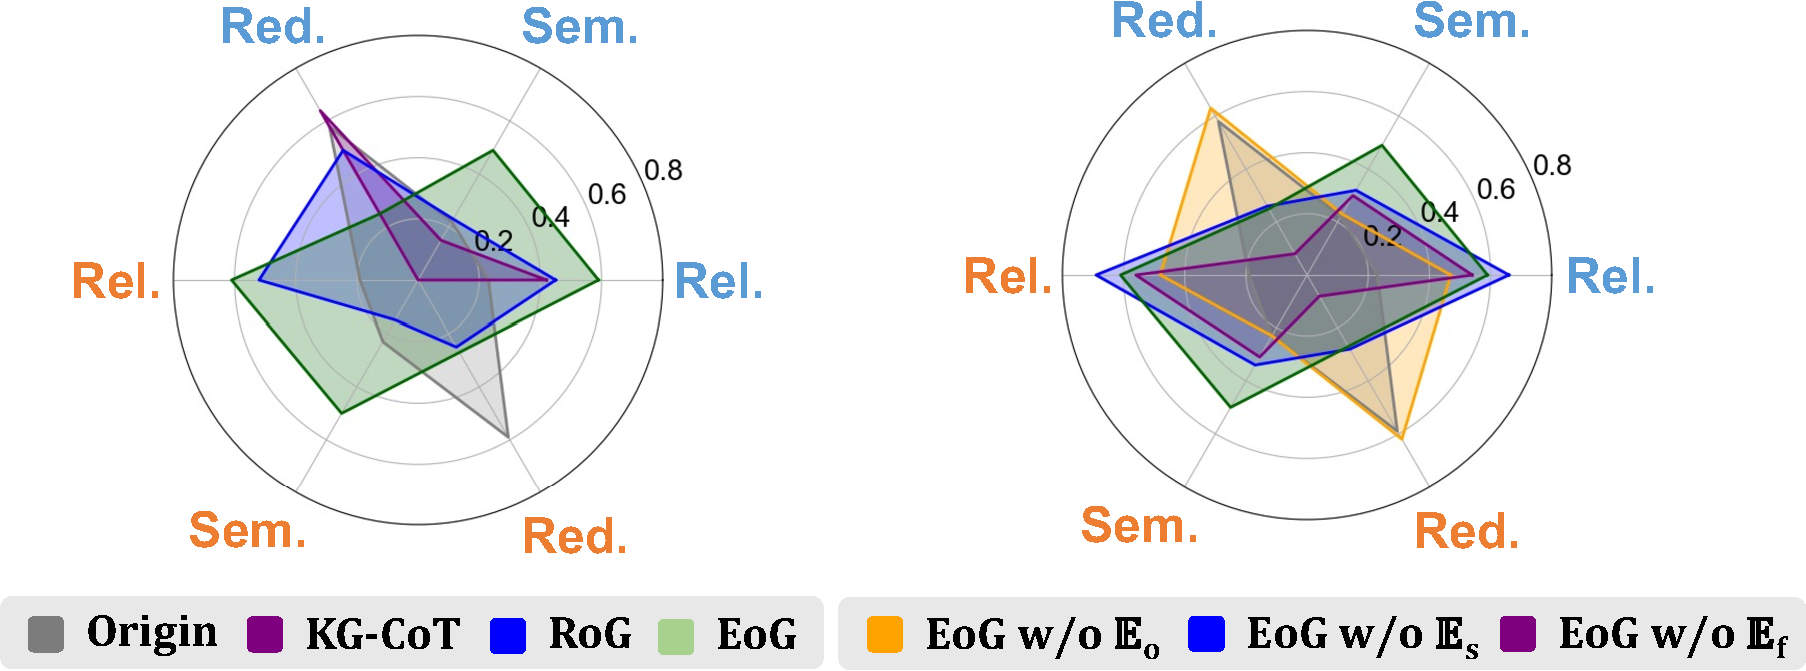
\includegraphics[width=\linewidth, keepaspectratio]{fig/combined_radar_charts.pdf}
    \caption{\textbf{Left:} Comparison of graph quality metrics between EoG and other methods.
\textbf{Right:} Validation of graph quality improvement by Prune and Enrich modules. \textbf{Rel.}, \textbf{Sem.}, and \textbf{Red.} indicate Relevance, Semantic richness, and Redundancy, respectively, and these metrics in the blue and orange respectively represent the results on the CWQ and WebQSP. }
    \label{graph metrics cmp}
\end{figure}


% To highlight the advantages of EoG-generated graphs over other KGQA methods, we visualize graph quality using three metrics: relevance, semantic richness, and redundancy. On the WebQSP and CWQ datasets, we compared EoG graphs with those from the original dataset, RoG, and KG-CoT. Since KG-CoT’s code is incompatible with WebQSP, we only report its results on CWQ (Fig.~\ref{graph metrics cmp} left).
% EoG achieves correlation scores above 0.6, significantly surpassing RoG and KG-CoT, indicating lower noise. Its semantic richness (\textasciitilde0.5) is over 20\% higher than other methods, demonstrating enhanced semantics for better LLM reasoning. EoG also records the lowest redundancy (\textasciitilde0.2), proving its graphs are concise with minimal irrelevant information.
% We further analyzed the impact of EoG’s core modules (Prune and Enrich) on graph quality (Fig.~\ref{graph metrics cmp} right). The Prune module significantly improves relevance by alleviating focus mismatches but does not mitigate redundancy. The Enrich module refines the graph by aligning structures with the query, drastically lowering redundancy. Both Feature Enrich and Structural Enrich enhance semantic richness and address the query-graph semantic gap. Feature Enrich adds ontology for entity disambiguation, nearly eliminating redundancy.

To showcase the advantages of EoG-generated graphs, we evaluated their quality using three metrics: relevance, semantic richness, and redundancy. On the WebQSP and CWQ datasets, EoG was compared with the original dataset, RoG, and KG-CoT. KG-CoT results are only reported for CWQ due to incompatibility with WebQSP (Fig.~\ref{graph metrics cmp} left).
EoG achieves relavance scores above 0.6, outperforming RoG and KG-CoT with less noise. Its semantic richness (\textasciitilde0.5) is 20\% higher, enhancing semantics for better LLM reasoning. Furthermore, EoG has the lowest redundancy (\textasciitilde0.2), ensuring concise graphs with minimal redundant information.
We also analyzed the effects of EoG’s Prune and Enrich modules (Fig.~\ref{graph metrics cmp} right). 
The results show that the Prune improves the relevance score by over 0.25. Structural Enrich and Feature Enrich each increase the semantic richness score by over 0.1, while their combination improves it by over 0.26. Feature Enrich significantly reduces redundancy to below 0.1. This demonstrates the contribution of Prune and Enrich in improving subgraph quality and aligning KGs with the query.
% Prune improves relevance by addressing focus mismatches but does not reduce redundancy. Enrich aligns graph structures with queries, significantly reducing redundancy. Feature Enrich and Structural Enrich both enhance semantic richness and tackle query-graph mismatches. Feature Enrich also adds ontology to disambiguate entities, nearly eliminating redundancy.

Additionally, we visualized random CWQ cases to illustrate EoG’s graph quality advantages across metrics in Fig.~\ref{fig:cwq graph quality visualization}.
\textbf{Relevance:} Using t-SNE, we plotted triples and question embeddings in 2D, with yellow dots marking question positions. EoG triples are closer and more concentrated around these points compared to the dispersed, noisy clusters of other methods, confirming higher relevance and reduced noise.
\textbf{Semantic Richness:} With t-SNE and KG-BERT semantic scoring, circle sizes represent triple semantic scores (larger circles denote higher scores). EoG covers a significantly larger total area, illustrating richer semantic information.
\textbf{Redundancy:} Triple redundancy was visualized as a density distribution of pairwise Euclidean distances. EoG triples exhibit greater spacing, indicating lower redundancy and more concise graphs. 
\begin{figure}[ht]
    \centering
    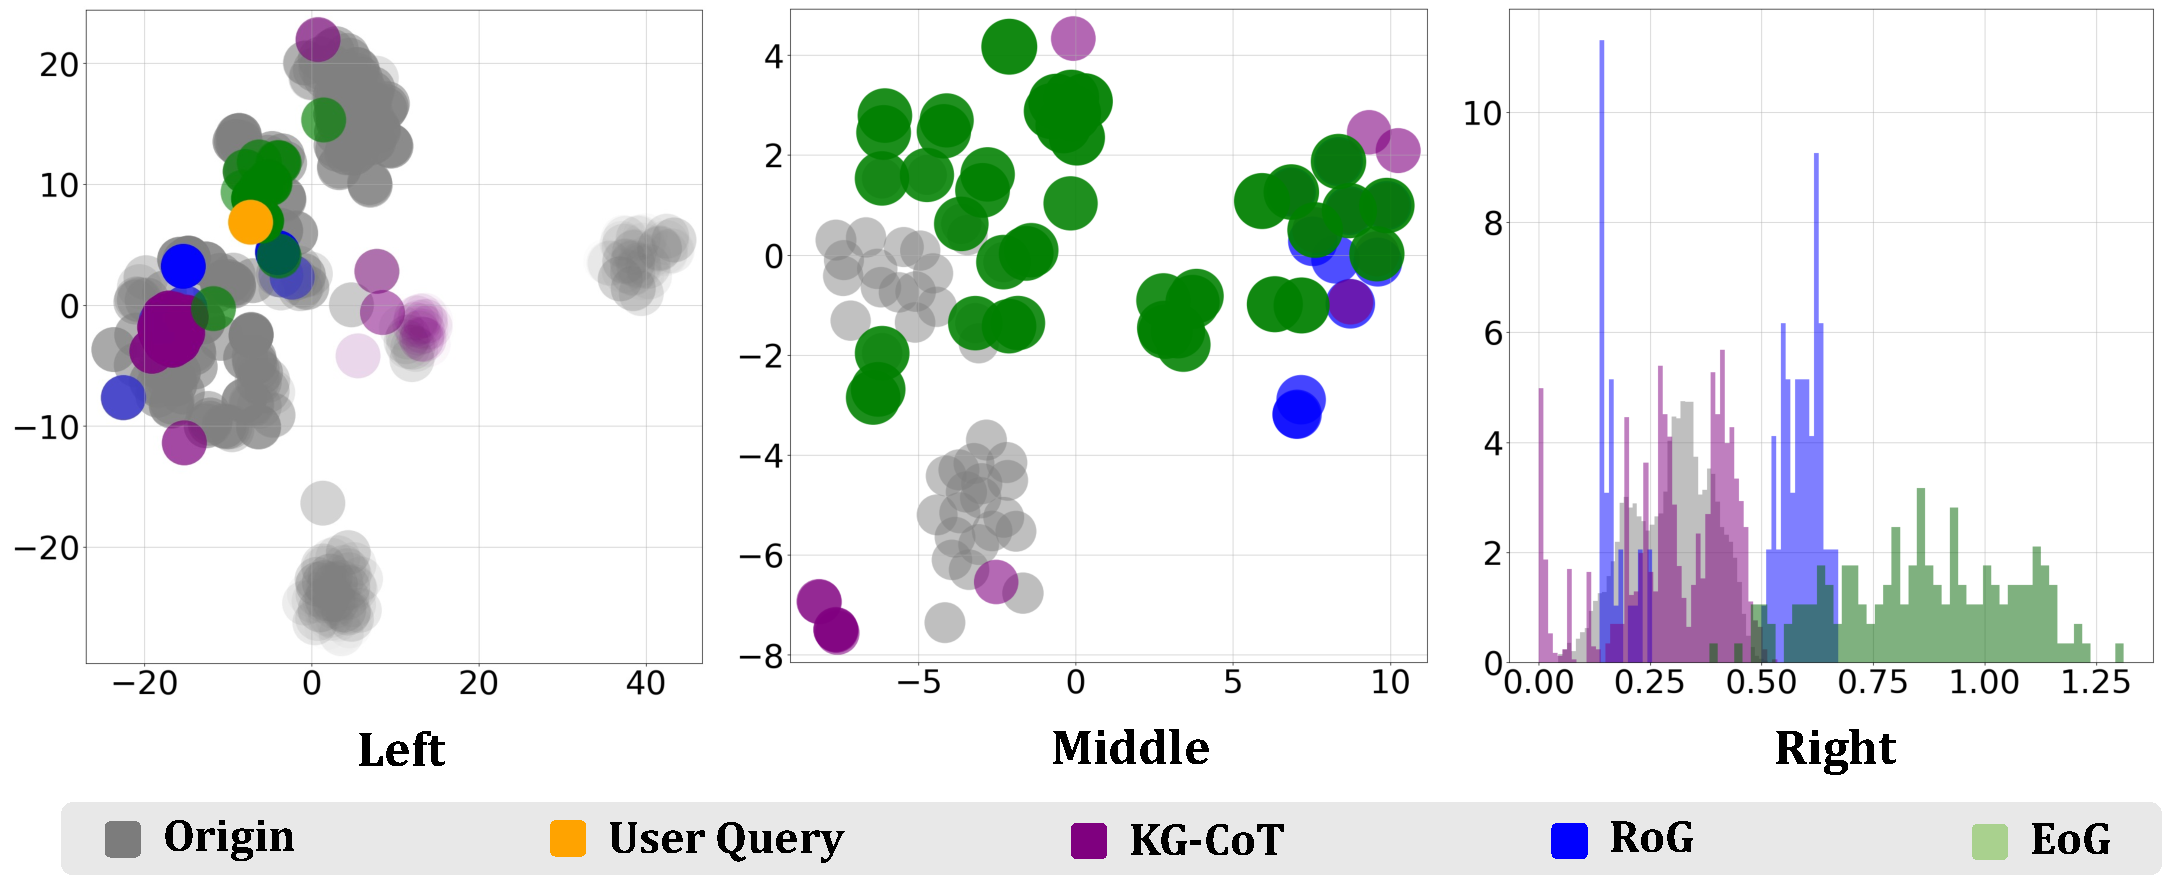
\includegraphics[width=\linewidth, keepaspectratio]{fig/merge_rel_sem_red.pdf}
    \caption{Graph visualization of EoG and advanced methods on the CWQ dataset.
\textbf{Left:} t-SNE projection of \textbf{Relevance}.
\textbf{Middle:} t-SNE visualization of \textbf{Semantic Richness}.
\textbf{Right:} Comparison of \textbf{Redundancy}.}
    \label{fig:cwq graph quality visualization}
\end{figure}


\subsection{Computation Cost}
\begin{table}[]
\resizebox{\linewidth}{!}{
\begin{tabular}{l|ccc|ccc}
\toprule
\multicolumn{1}{l|}{\multirow{2}{*}{Model}} & \multicolumn{3}{c|}{CWQ} & \multicolumn{3}{c}{WebQSP} \\ %\cline{2-7} 
\multicolumn{1}{c|}{} & \textit{\# LLM Call} & \textit{Total Token} & \textit{Total Cost} & \textit{\# LLM Call} & \textit{Total Token} & \textit{Total Cost} \\ \midrule
CoT & 1 & 409.7 & 8.00E-05 & 1 & 397.6 & 8.00E-05 \\
ToG & 9.2 & 11468.5 & 2.30E-03 & 8.8 & 10189.4 & 2.10E-03 \\
DoG & 5.7 & 37919.7 & 6.00E-03 & 2.7 & 6114.5 & 1.00E-03 \\ \midrule
EoG & 4 & 6213.6 & 1.10E-03 & 4 & 6802.1 & 1.20E-03 \\
w/o $\mathds{E}_o$ & 2 & 4610.0 & 7.00E-04 & 2 & 4841.6 & 8.00E-04 \\
w/o $\mathds{P}$ \& $\mathds{E}_o$ & 1 & 63814.4 & 9.00E-03 & 1 & 66928.0 & 1.00E-02 \\ \bottomrule
\end{tabular}
}
\caption{Efficiency comparison between EoG and other advanced methods.}
\label{computation cost}
\end{table}
We conducted a computation cost experiment to assess EoG's efficiency by comparing LLM call frequency, token usage, and cost metrics (Tab.~\ref{computation cost}). Results show EoG requires only 4 LLM calls per query, far fewer than ToG and DoG, and reduces token usage by 45.8\% and 83.6\% compared to ToG and DoG, respectively, with the lowest cost. Using the pruning module, EoG further cuts token usage by 92.8\%, highlighting its superior computational efficiency.
\subsection{Plug-and-Play}

\begin{table}[]
\centering
\resizebox{0.8\linewidth}{!}{
\begin{tabular}{l|llll}
\toprule
\multicolumn{1}{l|}{\multirow{2}{*}{Model}} & \multicolumn{2}{c}{CWQ\qquad} & \multicolumn{2}{l}{\quad WebQSP} \\ %\cline{2-5} 
\multicolumn{1}{c|}{} & \;\textit{Hit@1} & \textit{F1} & \textit{Hit@1} & \textit{F1} \\ \midrule
RoG & \;62.2 & 55.4 & 86.4 & 70.8 \\
RoG+$\mathds{E}_o$ & \;\textbf{75.4}\textsubscript{\textcolor{green}{↑13.2}} & \textbf{68.7}\textsubscript{\textcolor{green}{↑13.3}} & \textbf{91.5}\textsubscript{\textcolor{green}{↑5.1}} & \textbf{77.1}\textsubscript{\textcolor{green}{↑6.3}} \\ \midrule
KG-CoT & \;62.3 & 52.7 & \;\,- & \;\,- \\
KG-CoT+$\mathds{E}_o$ & \;\textbf{63.7}\textsubscript{\textcolor{green}{↑1.4}} & \textbf{65.7}\textsubscript{\textcolor{green}{↑13.0}} & \;\,- & \;\,- \\ \midrule
ToG & \;67.6 & \;\,- & 82.6 & \;\,- \\
ToG+$\mathds{E}_o$ & \;\textbf{70.7}\textsubscript{\textcolor{green}{↑3.1}} & \;\,- & \textbf{89.4}\textsubscript{\textcolor{green}{↑6.8}} & \;\,- \\ \midrule
DoG & \;56.0 & \;\,- & 91.0 & \;\,- \\
DoG+$\mathds{E}_o$ & \;\textbf{60.5}\textsubscript{\textcolor{green}{↑4.5}} & \;\,- & \textbf{92.5}\textsubscript{\textcolor{green}{↑1.5}} & \;\,- \\ \bottomrule
\end{tabular}
}
\caption{Impact of the Enrich module as a plugin enhancing other KGQA methods.}
\label{plug-and-play}
\end{table}

To validate EoG's plug-and-play capability, we applied the Enrich module to enhance other KGQA methods. As shown in Tab.~\ref{plug-and-play}, integrating Enrich with RoG, KG-CoT, ToG, and DoG significantly improved Hits@1 and F1, demonstrating its adaptability and robustness across KGQA methods. 
Additionally, experiments on base models with different reasoning capabilities and temperature parameters achieved excellent results, demonstrating EoG's strong reproducibility and plug-and-play flexibility (results in Appendix~\ref{plug-and-play-base-model}).

% \subsection{Case Study}
% We conducted a detailed case study on the CWQ dataset in Appendix~\ref{Case Study}, highlighting the semantic gap between the query and the vanilla KG, and \textit{\textbf{demonstrating how EoG-generated query-aligned graphs reduce reasoning complexity and enable LLMs to reason efficiently}}.

\section{Related Work}
\label{related work}

\paragraph{Traditional KGQA.}
Traditional KGQA methods are often categorized into information retrieval and semantic parsing approaches. Information retrieval methods (e.g., KV-Mem~\cite{miller-etal-2016-key}, GraftNet~\cite{DBLP:conf/emnlp/SunDZMSC18}, PullNet~\cite{sun-etal-2019-pullnet}, EmbedKGQA~\cite{saxena-etal-2020-improving}, NSM+h~\cite{10.1145/3437963.3441753}, TransferNet~\cite{shi-etal-2021-transfernet}, and Subgraph Retrieval~\cite{zhang-etal-2022-subgraph}) rely on retrieving query-relevant subgraphs from KGs but often retrieve irrelevant noises, leading to focus mismatch and reasoning errors. Semantic parsing (e.g., SPARQL~\cite{sun2020sparqaskeletonbasedsemanticparsing}, UHop~\cite{chen-etal-2019-uhop}, Topic Units~\cite{ijcai2019p701}, QGG~\cite{lan-jiang-2020-query}, UniKGQA~\cite{jiang2023unikgqa}, RnG-KBQA~\cite{ye-etal-2022-rng}, and TIARA~\cite{shu-etal-2022-tiara}) converts user queries into formal representations (e.g., SPARQL) to retrieve answers but struggles with complex queries, causing incomplete or failed answers.
\paragraph{LLMs for KGQA.}\vspace{-5pt}
LLMs introduce a transformative approach to KGQA, achieving state-of-the-art results through fine-tuned models and advanced prompting strategies. Earlier works leverage Flan-T5-xl~\cite{chung2022scalinginstructionfinetunedlanguagemodels}, Alpaca-7B~\cite{alpaca}, and LLaMa2-Chat-7B~\cite{touvron2023llama2openfoundation} with CoT (Chain-of-Thought)~\cite{wei2023chainofthoughtpromptingelicitsreasoning}, ToT (Tree-of-Thought)~\cite{yao2023treethoughtsdeliberateproblem}, and GoT (Graph-of-Thought)~\cite{Besta_2024} to enhance reasoning reliability, showcasing strong semantic understanding and reasoning abilities.
Advanced methods highlight these capabilities for KGQA but lead to resource-intensive workflows that lack scalability.
StructGPT~\cite{jiang2023structgptgeneralframeworklarge} unifies the discrepancies between queries and various data formats for collaborative reasoning. ReACT~\cite{yao2023reactsynergizingreasoningacting}, KD-CoT~\cite{wang2023knowledgedrivencotexploringfaithful}, DoG~\cite{ma2025debate}, and ToG~\cite{sun2023thinkongraph} iteratively decompose query and perform step-by-step reasoning while focusing on single-hop subgraphs. However, these methods face challenges such as complex workflows with iterative interactions and increased expenses. KG-CoT~\cite{inproceedings} and RoG~\cite{luo2024reasoninggraphsfaithfulinterpretable} plan relational paths based on the query and extract relevant relational subgraphs from vanilla KGs as external knowledge to assist LLMs, but they are limited to specific KGs and incur high training costs.

Most LLM-based KGQA methods attempt to align query-graph semantics through reasoning, but still face a semantic gap with vanilla KGs, hindering reasoning.

% Most LLM-based KGQA methods attempt to align the semantics between queries and graphs through reasoning, but they still suffer from the semantic gap when reasoning over vanilla KGs, which further impairs reasoning. 
% To overcome these issues, we propose using LLMs’ prior knowledge to enrich KGs, bridging semantic gaps and enhancing efficiency for complex KGQA tasks.

\section{Conclusion}
In this paper, we propose EoG, which leverages LLMs as priors to generate query-aligned graphs for efficient reasoning. For KGQA tasks, we identify the key insight of the semantic gap between queries and graphs and tackle the limitations of vanilla KGs while avoiding the complex reasoning pipeline of existing methods. We also introduce three graph evaluation metrics with theoretical support. Extensive experiments show EoG achieves SOTA performance in KGQA while maintaining low computational costs, scalability, and adaptability across different methods.
\section*{Limitations}
The limitations of our work at the current stage are mainly twofold:

(1) In the Feature Enrich part, we generate a general-domain ontology hierarchy. However, for tasks with varying ontology granularity across different domains, it may be necessary to design domain-specific ontology hierachy structures tailored to each domain.

(2) In our work, we use ChatGPT-series LLMs for query-graph alignment. Further exploration is needed to evaluate the alignment performance of LLMs with different parameter scales. In future work, we will investigate the performance of various LLMs at different parameter levels.
%\section*{Acknowledgments}

% Bibliography entries for the entire Anthology, followed by custom entries
%\bibliography{anthology,custom}
% Custom bibliography entries only

\section{Acknowledgement}

This work is founded by National Natural Science Foundation of China (NSFC62306276 / NSFCU23B2055 / NSFCU19B2027), Zhejiang Provincial Natural Science Foundation of China (No. LQ23F020017), Yongjiang Talent Introduction Programme (2022A-238-G), and Fundamental Research Funds for the Central Universities (226-2023-00138). This work was supported by Ant Group.

\bibliography{custom}

\section*{Appendix}
\label{sec:appendix}
\appendix
\section{Datasets Statistics}
\label{datastes statics}

We use two KGQA benchmarks that leverage Freebase~\cite{Bollacker2008FreebaseAC} as the underlying knowledge graph: WebQuestionSP~\cite{DBLP:conf/acl/YihRMCS16} and Complex WebQuestions~\cite{Talmor2018TheWA}. To ensure fair comparison, the dataset preprocessing follows previous work~\cite{luo2024reasoninggraphsfaithfulinterpretable}. Dataset statistics are provided in Tab.~\ref{Datasets statistics of WebQSP and CWQ}, which shows the dataset splits as well as the number of reasoning hops required to answer the questions. WebQSP contains 2,826 and 1,628 questions for the training and test sets, respectively, while CWQ consists of 27,639 and 3,531 questions for the training and test sets, respectively. In WebQSP, the questions mainly involve 1-hop and 2-hop reasoning, with 2-hop questions accounting for 34.51\%. CWQ includes questions requiring 1 to 4 hops, with those involving more than 2 hops making up 59.09\%. As shown in Tab.~\ref{Answer Distribution Proportion of WebQSP and CWQ}, both datasets contain multi-answer samples, with 48.8\% of WebQSP questions and 29.4\% of CWQ questions having two or more answers.

% Datasets statistics of WebQSP and CWQ
\begin{table}[H]
\resizebox{\linewidth}{!}{
\begin{tabular}{c|ccccccc}
\midrule
Datasets & KB & \#Train & \#Test & 1 hop & 2 hop & $\geq 3$ hop & Max \#hop \\ \midrule
WebQSP & Freebase & 2826 & 1628 & 65.49\% & 34.51\% & 0.00\% & 2 \\
CWQ & Freebase & 27639 & 3531 & 40.91\% & 38.34\% & 20.75\% & 4 \\ \midrule
\end{tabular}
}
\caption{Datasets statistics of WebQSP and CWQ}
\label{Datasets statistics of WebQSP and CWQ}
\end{table}

\begin{table}[H]
\centering
\resizebox{0.8\linewidth}{!}{
\begin{tabular}{c|cccc}
\midrule
Datasets & \#Ans=1 & 2 $\geq$ \#Ans $\leq$ & 5 $\geq$ \#Ans $\leq$ 9 & \#Ans $\geq$ 10 \\ \midrule
WebQSP & 51.20\% & 27.40\% & 8.30\% & 12.10\% \\
CWQ & 70.60\% & 19.40\% & 6\% & 4\% \\ \midrule
\end{tabular}
}
\caption{Answer distribution proportion of WebQSP and CWQ}
\label{Answer Distribution Proportion of WebQSP and CWQ}
\end{table}

\section{Prompts}
Listing~\ref{CoT Prompt},~\ref{Query Structuring Prompt},~\ref{Structural Enrich Prompt},~\ref{Feature Enrich Prompt},~\ref{Question Answering Prompt} detail the specific designs of the Chain of Thought prompt, Query Structuring prompt, Structural Enrich prompt, Feature Enrich prompt, and Question Answering prompt. For the CoT prompt, we directly adopt the design from~\cite{sun2023thinkongraph}. Due to space constraints, some demonstrations for the Structural Enrich prompt and Feature Enrich prompt are omitted.
\subsection{Chain of Thought Prompt}

\lstset{
    basicstyle=\ttfamily\fontsize{7}{8}\selectfont,
    breaklines=true,                  
    prebreak=\mbox{},               
    postbreak=\mbox{},              
    breakindent=0pt,               
    frame=single,                  
    tabsize=4,                      
    showstringspaces=false,   
    columns=fixed,           
    keepspaces=true,             
    captionpos=b,
}


\begin{lstlisting}[language=, caption={Demonstration of CoT Prompt}]
Q: What state is home to the university that is represented in sports by George Washington Colonials men's basketball?\nA: First, the education institution has a sports team named George Washington Colonials men's basketball in is George Washington University , Second, George Washington University is in Washington D.C. The answer is {Washington, D.C.}.

Q: Who lists Pramatha Chaudhuri as an influence and wrote Jana Gana Mana?
A: First, Bharoto Bhagyo Bidhata wrote Jana Gana Mana. Second, Bharoto Bhagyo Bidhata lists Pramatha Chaudhuri as an influence. The answer is {Bharoto Bhagyo Bidhata}.

Q: Who was the artist nominated for an award for You Drive Me Crazy?
A: First, the artist nominated for an award for You Drive Me Crazy is Britney Spears. The answer is {Jason Allen Alexander}.

Q: What person born in Siegen influenced the work of Vincent Van Gogh?
A: First, Peter Paul Rubens, Claude Monet and etc. influenced the work of Vincent Van Gogh. Second, Peter Paul Rubens born in Siegen. The answer is {Peter Paul Rubens}.

Q: What is the country close to Russia where Mikheil Saakashvii holds a government position?
A: First, China, Norway, Finland, Estonia and Georgia is close to Russia. Second, Mikheil Saakashvii holds a government position at Georgia. The answer is {Georgia}.

Q: What drug did the actor who portrayed the character Urethane Wheels Guy overdosed on?
A: First, Mitchell Lee Hedberg portrayed character Urethane Wheels Guy. Second, Mitchell Lee Hedberg overdose Heroin. The answer is {Heroin}.

Q: {question}
\end{lstlisting}
\label{CoT Prompt}


% \begin{figure}[ht]
% \centering
% \includegraphics[scale=0.35]{fig/cot_prompt.png}
% \vspace{-1mm}
% \caption{} \label{prompt1}
% \end{figure}

\subsection{Query Structuring Prompt}
\begin{lstlisting}[language=, caption={Demonstration of Query Structuring Prompt}]
[INST] <<SYS>>
<</SYS>>
{instruction}
Given a question, decompose it step by step into smaller components until it is broken down into unit queries that can be directly answered without further reasoning or decomposition. A unit query is a question that cannot be divided further and can be answered directly. If the given question is already a unit query, no decomposition is needed(If a question can still be further broken down, it must be divided into at least $two or more sub-questions$. Otherwise, the question is considered a unit query.). Your output should only include the tree structure of the decomposed question, with sub-questions indented using "-", and no additional content should be provided, just the tree structure. The format for the decomposition tree is as follows:
### decomposition tree format ###
question
-sub-question
--sub-sub-question
---sub-sub-sub-question
---sub-sub-sub-question
--sub-sub-question
-sub-question
### decomposition tree format ###
I will provide examples, please complete your task after reviewing them.
{/instruction}
{demonstrations}
### Example 1:
Input:
What is the name of the scientist who developed the theory that explains why objects fall to Earth?
Output:
What is the name of the scientist who developed the theory that explains why objects fall to Earth?
-What is the theory that explains why objects fall to Earth?
--Is there a theory for why objects fall to Earth?
--What is the name of this theory?
-Who developed this theory?
--Is this theory associated with a specific scientist?
--What is the name of this scientist?
### Example 2:
Input:
What type of energy powers the device invented by Thomas Edison that produces light?
Output:
What type of energy powers the device invented by Thomas Edison that produces light?
-What device produces light and was invented by Thomas Edison?
--Who is Thomas Edison?
--What devices did Thomas Edison invent?
--Is there a device invented by Thomas Edison that produces light?
--What is the name of this device?
-What type of energy powers this device?
--What is energy in this context?
--What is the primary mechanism or process that allows this device to produce light?
--What type of energy drives this mechanism?
### Example 3:
Input:
What inspired the author of the book "1984" to write it?
Output:
What inspired the author of the book "1984" to write it?
-Who is the author of the book "1984"?
--What is the book "1984"?
--Who wrote the book "1984"?
-What inspired this author to write "1984"?
--What was happening during the time this author wrote "1984"?
--What personal experiences influenced the author?
--What political or social events might have inspired the author?
--Did any other books or ideas inspire the author?
### Example 4:
Input:
What is the atomic number of the element discovered in the laboratory where the youngest Nobel Physics laureate worked?
Output:
What is the atomic number of the element discovered in the laboratory where the youngest Nobel Physics laureate worked?
-Who is the youngest Nobel Physics laureate?
--When did this person win the Nobel Prize?
--What was their age at the time of the award?
-Where did this laureate work?
--Did this laureate work in laboratory/institution?
--what's the name of the laboratory/institution?
-Was any chemical element discovered at this laboratory?
--What is the name of the element?
--What is its atomic number?
### Example 5:
Input:
Which country hosted the sporting event where the first female gold medalist in track and field competed?
Output:
Which country hosted the sporting event where the first female gold medalist in track and field competed?
-What type of sporting event is being referred to (e.g., Olympics)?
-Who was the first female gold medalist in track and field?
--What is track and field?
--Which female athlete won the first gold medal in this category?
-In which event within track and field did she win?
-Which country hosted this sporting event?
{/demonstrations}
### Your Turn
Input:
{question}
[/INST]
\end{lstlisting}
\label{Query Structuring Prompt}

\subsection{Structural Enrich Prompt}
\begin{lstlisting}[language=, caption={Demonstration of Structural Enrich Prompt}]
[INST] <<SYS>>You are a linguist capable of understanding user queries and the semantic information contained in triples. You can enhance the semantic information of triples based on the principles of similarity, symmetry, and transitivity, bridging the semantic gap between the triples and the user queries. Your goal is to augment the triples semantically so they can better address the user's queries.
<</SYS>>
{instruction}
You are given a subgraph that consists of multiple triples, where each triple corresponds to one or more user queries. The format is as follows:
triple(entity1, relation, entity2) - query1 - query2 - query3 - ...
Here, a query represents a question from the user. The triple associated with a query may contain information relevant to answering the question. However, the semantic connections both within and between triples are typically weak, lacking dense links to clearly establish relationships between entities. As a result, answers to the queries are often implicit and require complex reasoning. To bridge the semantic gap between the queries and the triples, please perform semantic enhancement on the subgraph by considering the user queries.
Specifically, you will utilize the following properties for semantic enhancement: Similarity, Symmetry, and Transitivity. Below, you will find detailed explanations of these properties along with examples. Please keep these principles in mind as you perform semantic enhancement.
{Similarity}
The property of similarity indicates that for a given triple (e1, r1, e2), we can find an alternative relationship r2 that is semantically different from r1 but shares the same directional connection between e1 and e2. In other words, the entities e1 and e2 remain connected in the same direction, but the meaning of the connection changes to reflect the semantics of r2. For example:
If (e1, r1, e2) exists, then (e1, r2, e2) may also exist, where r1 != r2, and r1 and r2 represent different relationships.
{/Similarity}
{Symmetry}
The property of symmetry indicates that for a given triple (e1, r1, e2), there exists a new relationship r2 that is semantically different from r1 and reverses the direction of the connection between e1 and e2. In other words, the new triple swaps the roles of e1 and e2 while preserving their semantic relationship in a reversed form. For example:
If (e1, r1, e2) exists, then (e2, r2, e1) may also exist, where r1 != r2, and r1 and r2 represent different relationships.
{/Symmetry}
{Transitivity}
The property of transitivity indicates that when two triples share a common entity, we can combine their relationships into a new relationship that connects the remaining two entities directly. Specifically, if (e1, r1, e2) and (e2, r2, e3) exist, then there exists a new relationship r3 that semantically encompasses both r1 and r2, forming a new triple (e1, r3, e3). The new relationship r3 captures the combined semantics of r1 and r2. For example:
Given (e1, r1, e2) and (e2, r2, e3), we derive (e1, r3, e3), where r3 combines the meanings of r1 and r2.
{/Transitivity}
Your task will follow the four steps below:
{Procedure}
Step 1:
Examine the given triples and their associated queries. Understand the information contained within the triples and the questions being asked in the queries.
Step 2:
Using the similarity and symmetry properties, perform semantic enhancement on the given 1-hop subgraph (i.e., triples where connections involve only directly linked entities).
Step 3:
Using the transitivity property, perform semantic enhancement on the given multi-hop subgraph (i.e., triples where connections involve intermediary entities).
Step 4:
Output the newly generated triples resulting from the semantic enhancement process.
{/Procedure}
I will provide examples, please complete your task after reviewing them.
{/instruction}
{demonstrations}
### Example 1:
Input:
(Michelle Bachelet,people.person.nationality,Chile)-What is the location that appointed Michelle Bachelet to a governmental position?-Who is Michelle Bachelet?-What governmental position was Michelle Bachelet appointed to?-Where was Michelle Bachelet appointed to this position?
(Chile,language.human_language.countries_spoken_in,Spanish Language)-What language is spoken in this location?
1-hop:
(Michelle Bachelet,people.person.nationality,Chile)
2-hop:
(Michelle Bachelet,people.person.nationality,Chile)->(Chile,language.human_language.countries_spoken_in,Spanish Language)
Output:
{thought}
step 1:
To prepare for the subsequent semantic enhancement of the triples and bridge the semantic gap between the triples and the user queries, let me review the triples along with their corresponding user query(ies):
(Michelle Bachelet,people.person.nationality,Chile)-What is the location that appointed Michelle Bachelet to a governmental position?-Who is Michelle Bachelet?-What governmental position was Michelle Bachelet appointed to?-Where was Michelle Bachelet appointed to this position?
(Chile,language.human_language.countries_spoken_in,Spanish Language)-What language is spoken in this location?
step 2:
Using the similarity property, perform semantic enhancement on the given 1-hop subgraph:
For the 1-hop subgraph (Michelle Bachelet,people.person.nationality,Chile),the related queries are "What is the location that appointed Michelle Bachelet to a governmental position?" , "Who is Michelle Bachelet?" , "What governmental position was Michelle Bachelet appointed to?" , "Where was Michelle Bachelet appointed to this position?" .Combining these queries, The newly added  triple(s) is/are (Michelle Bachelet,appointed_government_position_in,Chile)
Using the symmetry properties, perform semantic enhancement on the given 1-hop subgraph:
For the 1-hop subgraph (Michelle Bachelet,people.person.nationality,Chile),the related queries are "What is the location that appointed Michelle Bachelet to a governmental position?" , "Who is Michelle Bachelet?" , "What governmental position was Michelle Bachelet appointed to?" , "Where was Michelle Bachelet appointed to this position?" .Combining these queries, The newly added  triple(s) is/are (Chile, appointed_as_government_official_by, Michelle Bachelet)
step 3:
Using the transitivity properties, perform semantic enhancement on the given 2-hop subgraph:
For the 2-hop subgraph (Michelle Bachelet,people.person.nationality,Chile)->(Chile,language.human_language.countries_spoken_in,Spanish Language),the related queries are "What is the location that appointed Michelle Bachelet to a governmental position?" , "Who is Michelle Bachelet?" , "What governmental position was Michelle Bachelet appointed to?" , "Where was Michelle Bachelet appointed to this position?" , What language is spoken in this location?. Combining these queries, The newly added  triple(s) is/are (Michelle Bachelet, language_of_the_country_where_appointed ,Spanish Language)
step 4:
Final output:
(Michelle Bachelet,appointed_government_position_in,Chile)
(Chile, appointed_as_government_official_by, Michelle Bachelet)
(Michelle Bachelet, language_of_the_country_where_appointed ,Spanish Language)
{/thought}
...
{/demonstrations}
### Your Turn
Input:
{quadruples}
1-hop:
{1-hop path}
2-hop:
{2-hop path}
[/INST]
\end{lstlisting}
\label{Structural Enrich Prompt}

\subsection{Feature Enrich Prompt}
\begin{lstlisting}[language=, caption={Demonstration of Feature Enrich Prompt}]
[INST] <<SYS>>You are a linguist with extensive expertise in ontology knowledge. You have the ability to understand the context of entities, including user queries and the semantic information of triples. Based on the contextual information of an entity, you can accurately and appropriately add ontologies to the entity. Your goal is to bridge the semantic gap between entities and user queries by adding relevant ontologies, thereby semantically augmenting the entities to enable them to better address the user's queries.
<</SYS>>
{instruction}
You are provided with an entity list. Each entity in the list is accompanied by its context information, which consists of two parts:
1.Relevant triples associated with the entity.
2.Relevant user queries associated with the entity.
The context format for each entity is as follows:
[$entity$ context]
relavent triple(s):triple1-triple2-triple3-...
relavent user query(ies):query1-query2-query3-...
[/$entity$ context]
Your task is to analyze the context information of each entity, apply your expert knowledge, and assign an appropriate ontology to the entity. The added ontology should:
1.Be semantically consistent with the entity's context information.
2.Avoid any contradictions or irrelevance with the given context.
3.Enhance the entity's ability to better answer the user query(ies) in its context.
Store the ontology assignments in a set called {result}. The {result} set is initially empty. Each ontology assignment should follow the format:
{result}
(entity,ontology_relation,newly added ontology)
...
{/result}
You must choose an appropriate ontology relation from the options provided below.
{ontology relation definition}
HYP: Hypernym relation
Refers to the relation where a broader or more general concept includes or encompasses a more specific or specialized concept.
Hypernym_isA
Is a type of...
Hypernym_locateAt
Is located at...
Hypernym_mannerOf 
A is a specific implementation or way of B. Similar to "isA," but used for verbs. For example, "auction" -> "sale"
IND: Induction relation
Refers to the relation between individual entities and conceptual generalizations derived from a class of entities with common characteristics. 
Induction_belongTo
This relation is commonly used in SPG to describe the classification relation from entity types to concept types. For example, "company event" -> "company event category".
INC: Inclusion relation
Expresses the relation between parts and the whole. 
Inclusion_isPartOf
A is a part of B.
Inclusion_madeOf
A is made up of B. For example, "bottle" -> "plastic". 
Inclusion_derivedFrom
A is derived from or originated from B, used to express composite concepts.
Inclusion_hasContext
A is a word used in the context of B, where B can be a subject area, technical field, or regional dialect. For example, "astern" -> "ship".
{/ontology relation definition}
You can only choose an appropriate {ontology_relation} from {Hypernym_isA, Hypernym_locateAt, Hypernym_mannerOf, Induction_belongTo, Inclusion_isPartOf, Inclusion_madeOf, Inclusion_derivedFrom, Inclusion_hasContext}.
Your task will follow the four steps below:
{Procedure}
step 1:
For the first $entity$ in the entity list, read its context information carefully. Based on the provided context and your expert knowledge, answer the following question:
Does this $entity$ already have an ontology assigned?
If yes, proceed to Step 2.
If no, move to Step 3.
step 2:
Using the entity's context information and your expert knowledge:
Identify a list of appropriate ontologies for the entity.
For each ontology in this list, select the most suitable ontology relation from the {ontology_relation} options.
Format each assignment as (entity, ontology_relation, newly added ontology) and add it to the {result} set.
Remove this $entity$ and its corresponding context information from the entity list.
Output the current {result} set in the following format:
{result}
...
{/result}
Then move to Step 3.
step 3:
Check if the entity list is now empty:
If the list is empty, proceed to Step 4.
If the list is not empty, return to Step 1 and repeat the process for the next $entity$.
step 4:
Once all entities have been processed, output the final {result} set containing all (entity, ontology_relation, newly added ontology) assignments in the following format:
{result}
(entity,ontology_relation,newly added ontology)
...
{/result}
{/Procedure}
I will provide examples, please complete your task after reviewing them.
{/instruction}
{demonstrations}
### Example 1:
Input:
entity List:
[$Michelle Bachelet$ context]
relavent triple(s):(Michelle Bachelet,people.person.nationality,Chile)
relavent user query(ies):What is the location that appointed Michelle Bachelet to a governmental position?-Who is Michelle Bachelet?-What governmental position was Michelle Bachelet appointed to?-Where was Michelle Bachelet appointed to this position?
[/$Michelle Bachelet$ context]
[$Chile$ context]
relavent triple(s):(Michelle Bachelet,people.person.nationality,Chile)-(Chile,language.human_language.countries_spoken_in,Spanish Language)
relavent user query(ies):What is the location that appointed Michelle Bachelet to a governmental position?-Who is Michelle Bachelet?-What governmental position was Michelle Bachelet appointed to?-Where was Michelle Bachelet appointed to this position?-What language is spoken in this location?
[/$Chile$ context]
Output:
{result}
(Michelle Bachelet, Hypernym_isA, Political Figure)
(Michelle Bachelet, Hypernym_isA, President)
(Chile, Hypernym_isA, Country)
(Chile, Hypernym_locateAt, South America)
(Chile, Inclusion_hasContext, Spanish Language)
{/result}
...
{/demonstrations}
### Your Turn
Input:
entity List:
[$entity$ context]
relavent triple(s):
relavent user query(ies):
[/$entity$ context]
[/INST]
\end{lstlisting}
\label{Feature Enrich Prompt}

\subsection{Question Answering Prompt}
\begin{lstlisting}[language=, caption={Demonstration of Question Answering Prompt}]
[INST] <<SYS>>
<</SYS>>
{instruction}
You are given an input question along with additional information to assist in answering the question. The additional information includes a set of relevant triples. The format of a triple is as follows: 
(e1, r, e2)
Your task is to perform step-by-step reasoning based on the provided additional information to arrive at the answer. You should output your process of thinking and reasoning then the final answer. Each answer should be as close to a single entity as possible, rather than a long sentence. Each answer should not be in the form of an ID, such as: "m.0n1v8cy", "m.0jx21d", or similar formats. If the provided information is insufficient to infer the correct answer, please use your internal knowledge to generate a response. Please try to output all possible answers you consider correct. If there is only one answer, directly output that answer. If there are multiple answers, separate them using <SEP>.
### Input Format ###
Input:  
question:
{input question}  
information:
{triple1}
{triple2}
{triple3}
...
### Output Format ###
Output:
{thoughts & reason}
Your process of thinking and reasoning
...
{/thoughts & reason}
Final answer:
{answer}
{/instruction}
### Your Turn
Input:
question:
{question}
information:
{knowledge graph}
[/INST]
\end{lstlisting}
\label{Question Answering Prompt}

\section{Details of our Theoretical Proof}
\label{Details of our Theoretical Proof}
In this section, we provide a detailed derivation of the solution for EoG.

As stated in~\ref{theorem1}, our goal is to find an optimized graph $  G^*  $ by maximizing the expected posterior probability:

\[{G^{*} = \underset{G}{argmax}}{~\mathbb{E}_{P(q,G)}\left\lbrack P\left( M_{\theta},q \middle| G \right) \right\rbrack}\]

It is equivalent to maximizing the mutual information between $  q  $ and $  G  $.
The detailed derivation is as follows.

Since $  P(q)  $ and $  P(G)  $ are constants, we have:

{\small
\[P\left( M_{\theta},q \middle| G \right) \propto {\log\left( \frac{P\left( M_{\theta},q \middle| G \right)}{P(q)} \right)}\]
}

The equivalent transformation of the conditional probability is:

{\small
\[P\left( M_{\theta},q \middle| G \right) = \frac{P\left( M_{\theta},G \middle| q \right)P(q)}{P(G)}\]
}

We can obtain:

{\small
\[P\left( M_{\theta},q \middle| G \right) \propto {\log\left( \frac{P\left( M_{\theta},q \middle| G \right)}{P(q)} \right)}\]
}
{\small

\[{{= \log}\left( \frac{P\left( M_{\theta},G \middle| q \right)}{P(G)} \right)}\]

}

We eliminate the variable $  M_\theta  $ using the marginalization formula:

{\small
\[{\mathit{\log}\left( \frac{P\left( M_{\theta},G \middle| q \right)}{P(G)} \right)} \propto {\mathit{\log}\left( \frac{\int_{M_{\theta}}^{}{P\left( M_{\theta},G \middle| q \right)dM_{\theta}}}{P(G)} \right)}\]
}

We can obtain:

{\small

\[{\mathit{\log}\left( \frac{\int_{M_{\theta}}^{}{P\left( M_{\theta},G \middle| q \right)dM_{\theta}}}{P(G)} \right)} = \mathit{\log}\left( \frac{P\left( G \middle| q \right)}{P(G)} \right)\]

}

{\small

\[= {\log\left( \frac{P\left( {q,G} \right)}{P(q)P(G)} \right)}\]

}
Thus, the expectation of the original posterior probability is equivalent to:

{\small

\[\mathbb{E}_{P(Q,G)}\left\lbrack P\left( M_{\theta},q \middle| G \right) \right\rbrack \propto \mathbb{E}_{P(q,G)}\left\lbrack {\log\left( \frac{P\left( {q,G} \right)}{P(q)P(G)} \right)} \right\rbrack\]

}

Finally we can get:

\[\mathbb{E}_{P(q,G)}\left\lbrack {P\left( M_{\theta},q \middle| G \right)} \right\rbrack \propto MI(q,G)\]

\section{Optimal k-value Exploration}
\label{Optimal k-value Exploration}
To explore the optimal number of retrieved triples(\textit{k}) as discussed in Section~\ref{Structure-Aware Multi-Channel Pruning}, and to demonstrate the superiority of our Structure-Aware Multi-Channel Pruning method compared to the vanilla pruning approach, we evaluated the impact of different numbers of retrieved triples on \textbf{Answer Coverage} and \textbf{Token Cost} (using the default GPT-4o-mini) on the WebQSP and CWQ datasets.
For answer coverage, it is calculated as: \# Answers in Pruned Graph / \# Total Answers. For Token Cost, it is determined by converting triples directly into natural language text, e.g., converting (\textit{Beijing, located in, China}) into \textit{Beijing located in China}. We then compute the total token number of the converted text and multiply it by the OpenAI API price to get the token cost. The results are shown in Fig.~\ref{fig:k cwq} and Fig.~\ref{fig:k webqsp}, where the values represented by the green dashed lines indicate the answer coverage before pruning performed by~\cite{luo2024reasoninggraphsfaithfulinterpretable} on the dataset.
As the number of retrieved triples increases, the number of answers mistakenly removed by pruning decreases, but the token length grows, leading to a continuous increase in API invocation costs. When the number of retrieved triples is 300, the pruned graph obtained by Structure-Aware Multi-Channel Pruning has only a 5\% reduction in answer coverage compared to the unpruned graph. Compared to the vanilla pruning method, our pruning strategy achieves approximately 7\% higher answer coverage across all triple counts, which demonstrates the superiority of our approach.

Considering the trade-off between token cost and answer coverage, we chose $k=300$ as the optimal number of retrieved triples.

\begin{figure}[h!]
    \centering
    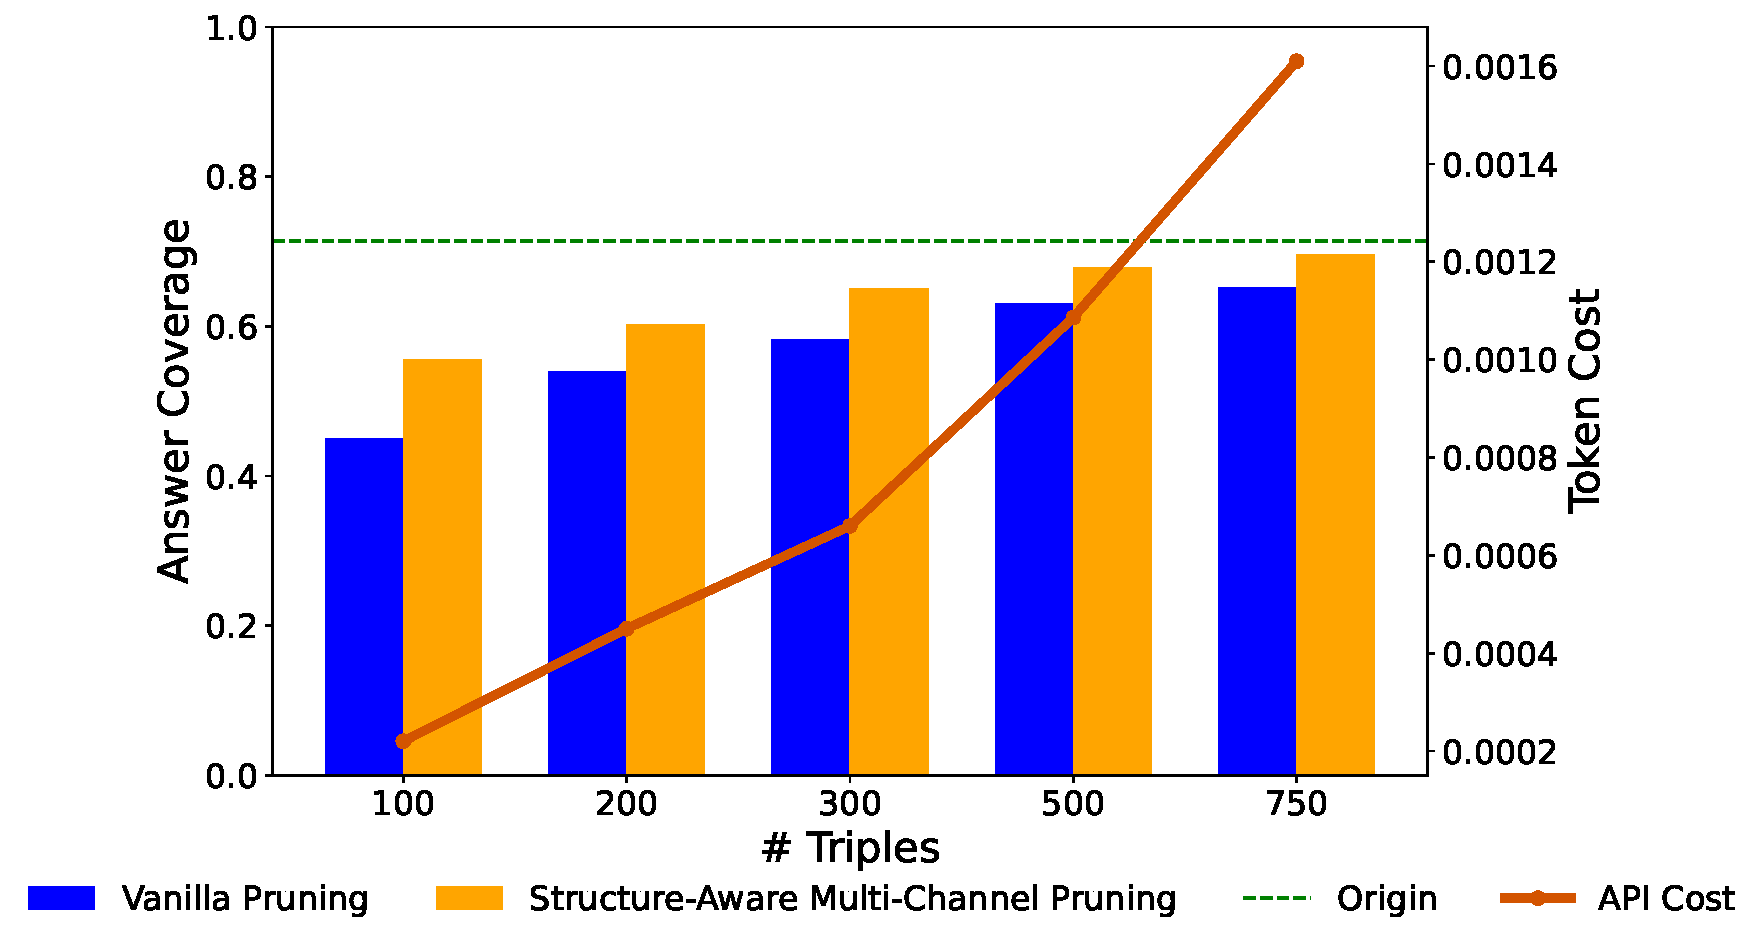
\includegraphics[width=\linewidth, keepaspectratio]{fig/k_visualization_cwq.pdf}
    \caption{Impact of the Number of Retrieved Triples on Answer Coverage Ratio and API Call Cost (\$) in the CWQ Dataset}
    \label{fig:k cwq}
\end{figure}

\begin{figure}[h!]
    \centering
    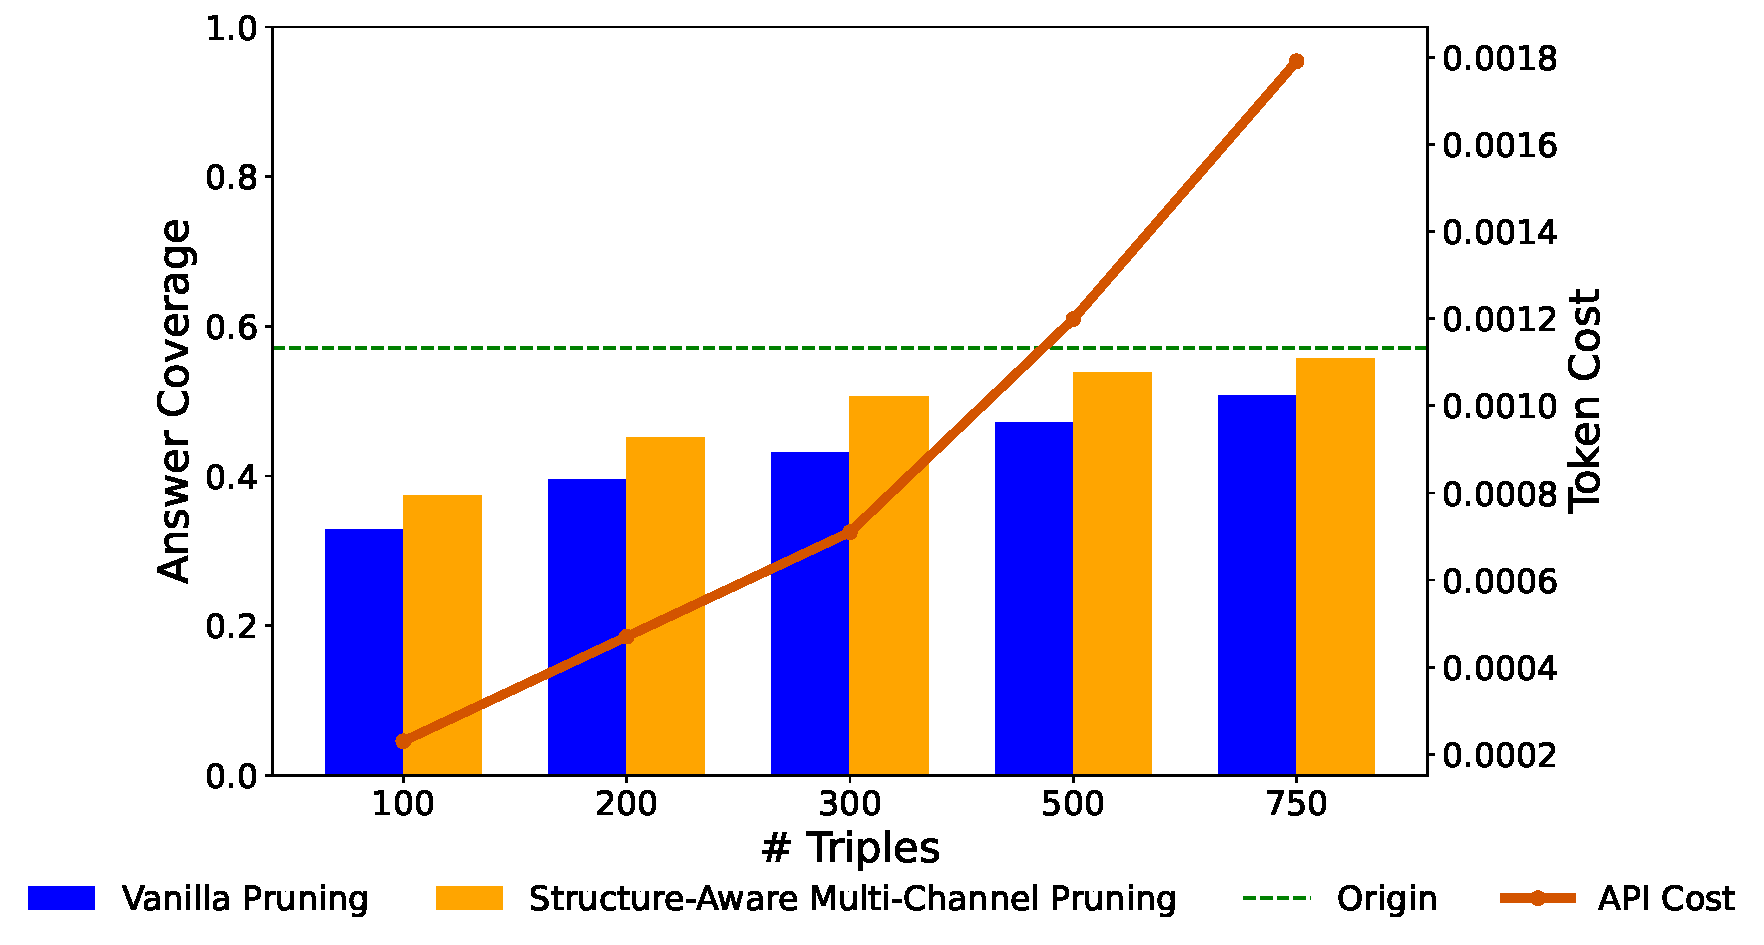
\includegraphics[width=\linewidth, keepaspectratio]{fig/k_visualization_webqsp.pdf}
    \caption{Impact of the Number of Retrieved Triples on Answer Coverage Ratio and API Call Cost (\$) in the WebQSP Dataset}
    \label{fig:k webqsp}
\end{figure}

\section{Case Study}
\label{Case Study}

In this section, we present case study on the CWQ dataset to illustrate the critical role of EoG-generated query-aligned graphs in reasoning. We provide two examples, as shown in Fig.~\ref{fig:case1} and Fig.~\ref{fig:case2}, comparing the performance of EoG with the vanilla KG method that assists ChatGPT in step-by-step reasoning. In the figures, green highlights the correct answers or key triples, red indicates misleading triples, and orange represents triples relevant to the query.

In the first example, the query is \textit{What is the currency of the place whose religious organization leadership is the Society of Jesus?} The retrieved triples include misleading information: (\textit{Pope Francis}, \textit{people.person.birth}, \textit{Italy}), (\textit{Italy}, \textit{location.country.currency\_used}, \textit{Euro}).
Using the vanilla KG, ChatGPT retrieves the entity \textit{m.0rgks1y} related to \textit{Society of Jesus}, but since it cannot interpret the entity's semantics, it overlooks the correct triple: (\textit{m.0rgks1y}, \textit{religion.religious\_organization\_leadership.jurisdic} \textit{tion, Argentina}). Additionally, (\textit{m.0rgks1y}, \textit{religion.religious\_organization\_leadership.leader}, \textit{Pope Francis}), (\textit{Pope Francis}, \textit{people.person.birth}, \textit{Italy}), and (\textit{Italy}, \textit{location.country.currency\_used}, \textit{Euro}) lead ChatGPT to assume that Pope Francis, as a leader of the Society of Jesus, is the key to solving the query and conclude that the answer is Euro based on Pope Francis’ birthplace, Italy. This error highlights the semantic gap between the query and the vanilla KG, resulting in incorrect reasoning.
EoG bridges this semantic gap by leveraging structural and feature attributes like similarity, symmetry, transitivity, and hierarchy. Through symmetry, EoG generates the triple: (\textit{m.0rgks1y}, \textit{religion.religious\_organization\_lead-}\newline 
\textit{ership.organization}, \textit{Society of Jesus}), indicating the leadership relationship between \textit{Society of Jesus} and \textit{m.0rgks1y}. Hierarchy generates: (\textit{m.0rgks1y}, \textit{Hypernym\_isA}, \textit{Religious Organization}), clarifying the meaning of \textit{m.0rgks1y}. Transitivity further establishes the relationship: (\textit{Society of Jesus}, \textit{religious\_leadership\_of\_place}, \textit{Argentina}), which aligns semantically with the query, reduces reasoning hops, and enables LLMs to correctly infer that \textit{Society of Jesus} is based in \textit{Argentina}. Finally, the hierarchical triple: (\textit{Argentina}, \textit{Inclusion\_hasContext}, \textit{Argentine Peso}) helps the LLM deduce that the currency of \textit{Argentina} is \textit{Argentine Peso}. This proves that EoG’s query-aligned graph effectively bridges the semantic gap, simplifies reasoning complexity, and enhances LLM efficiency.

\begin{figure*}[ht]
    \centering
    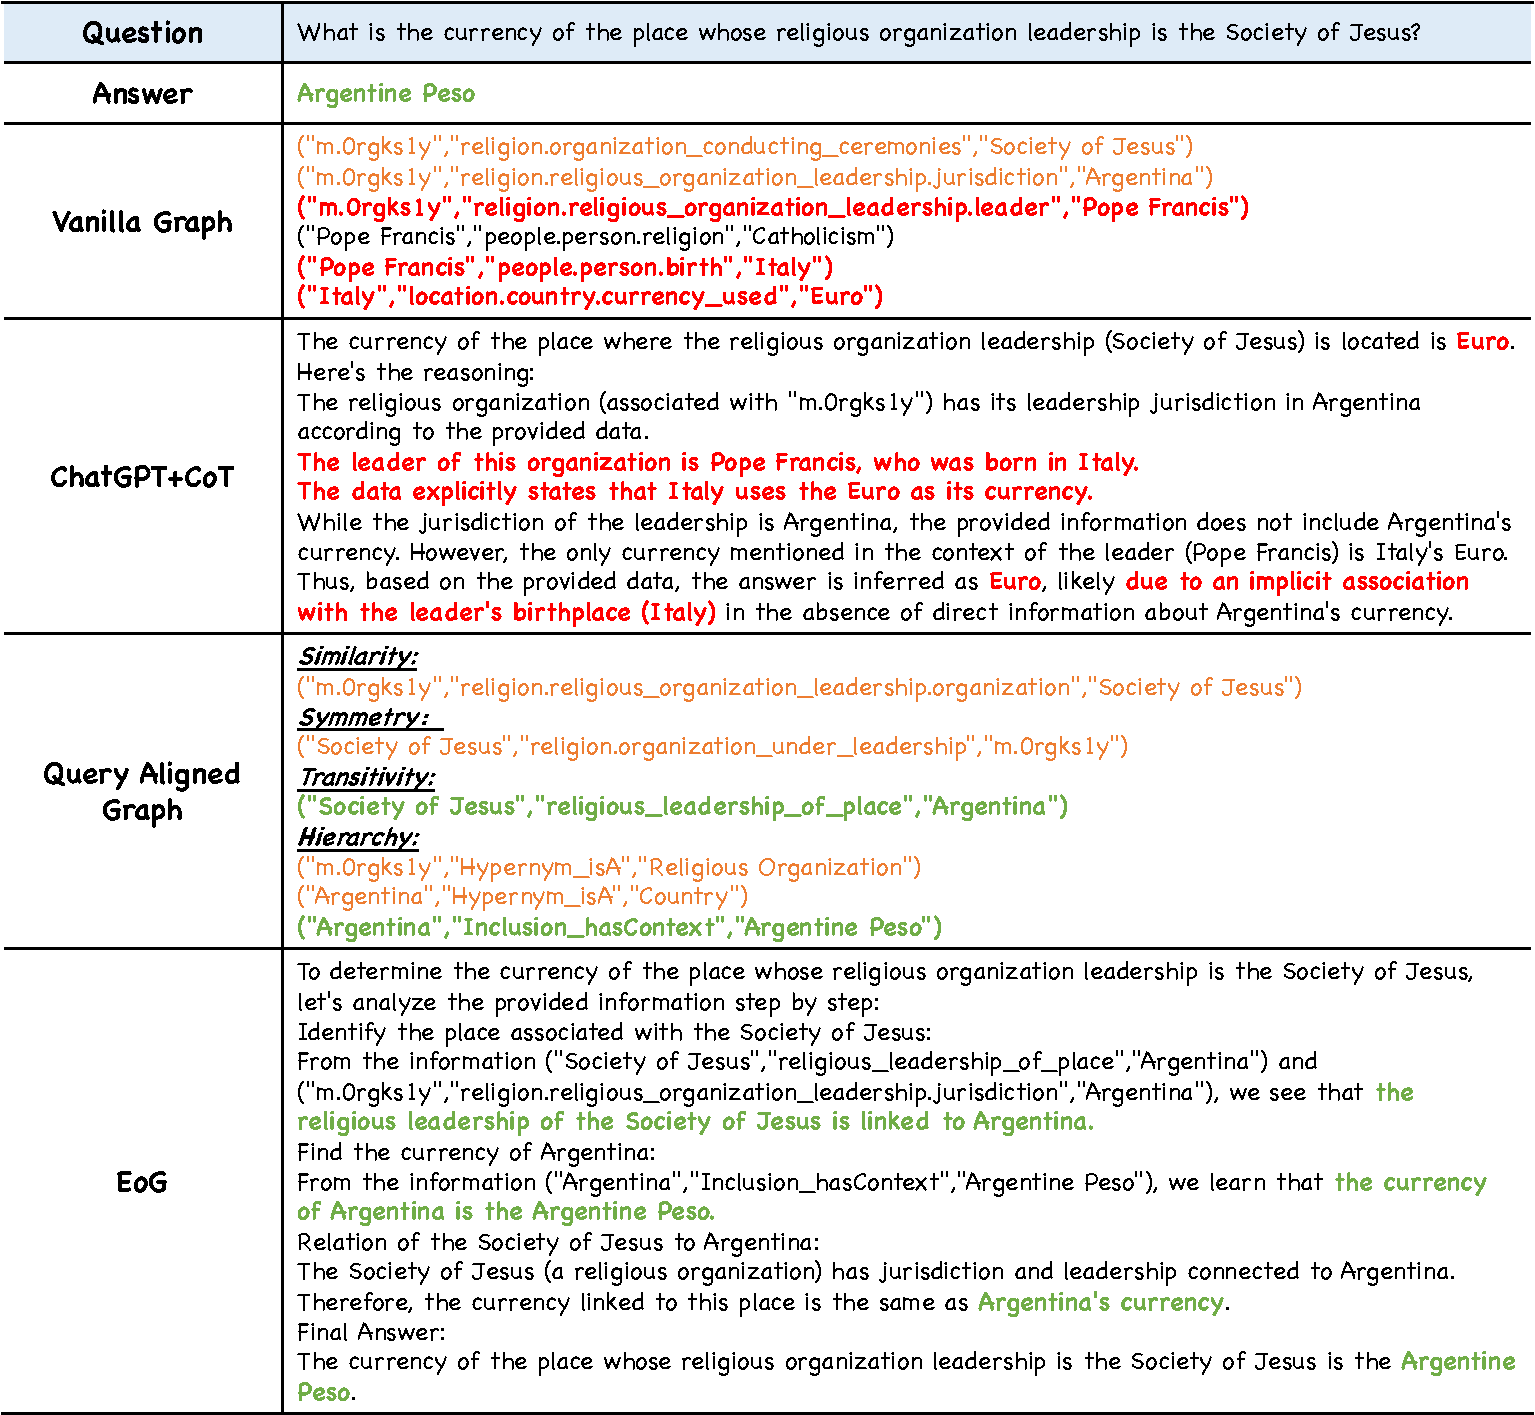
\includegraphics[width=\textwidth, keepaspectratio]{fig/case1.pdf}
    \caption{Case for EoG. \textbf{Green} highlights the correct answers or key triples, \textbf{Red} indicates misleading triples, and \textbf{Orange} represents triples relevant to the query.}
    \label{fig:case1}
\end{figure*}

% Case for EoG. Green highlights the correct answers or key triples, red indicates misleading triples, and orange represents triples relevant to the query.
\begin{figure*}[ht]
    \centering
    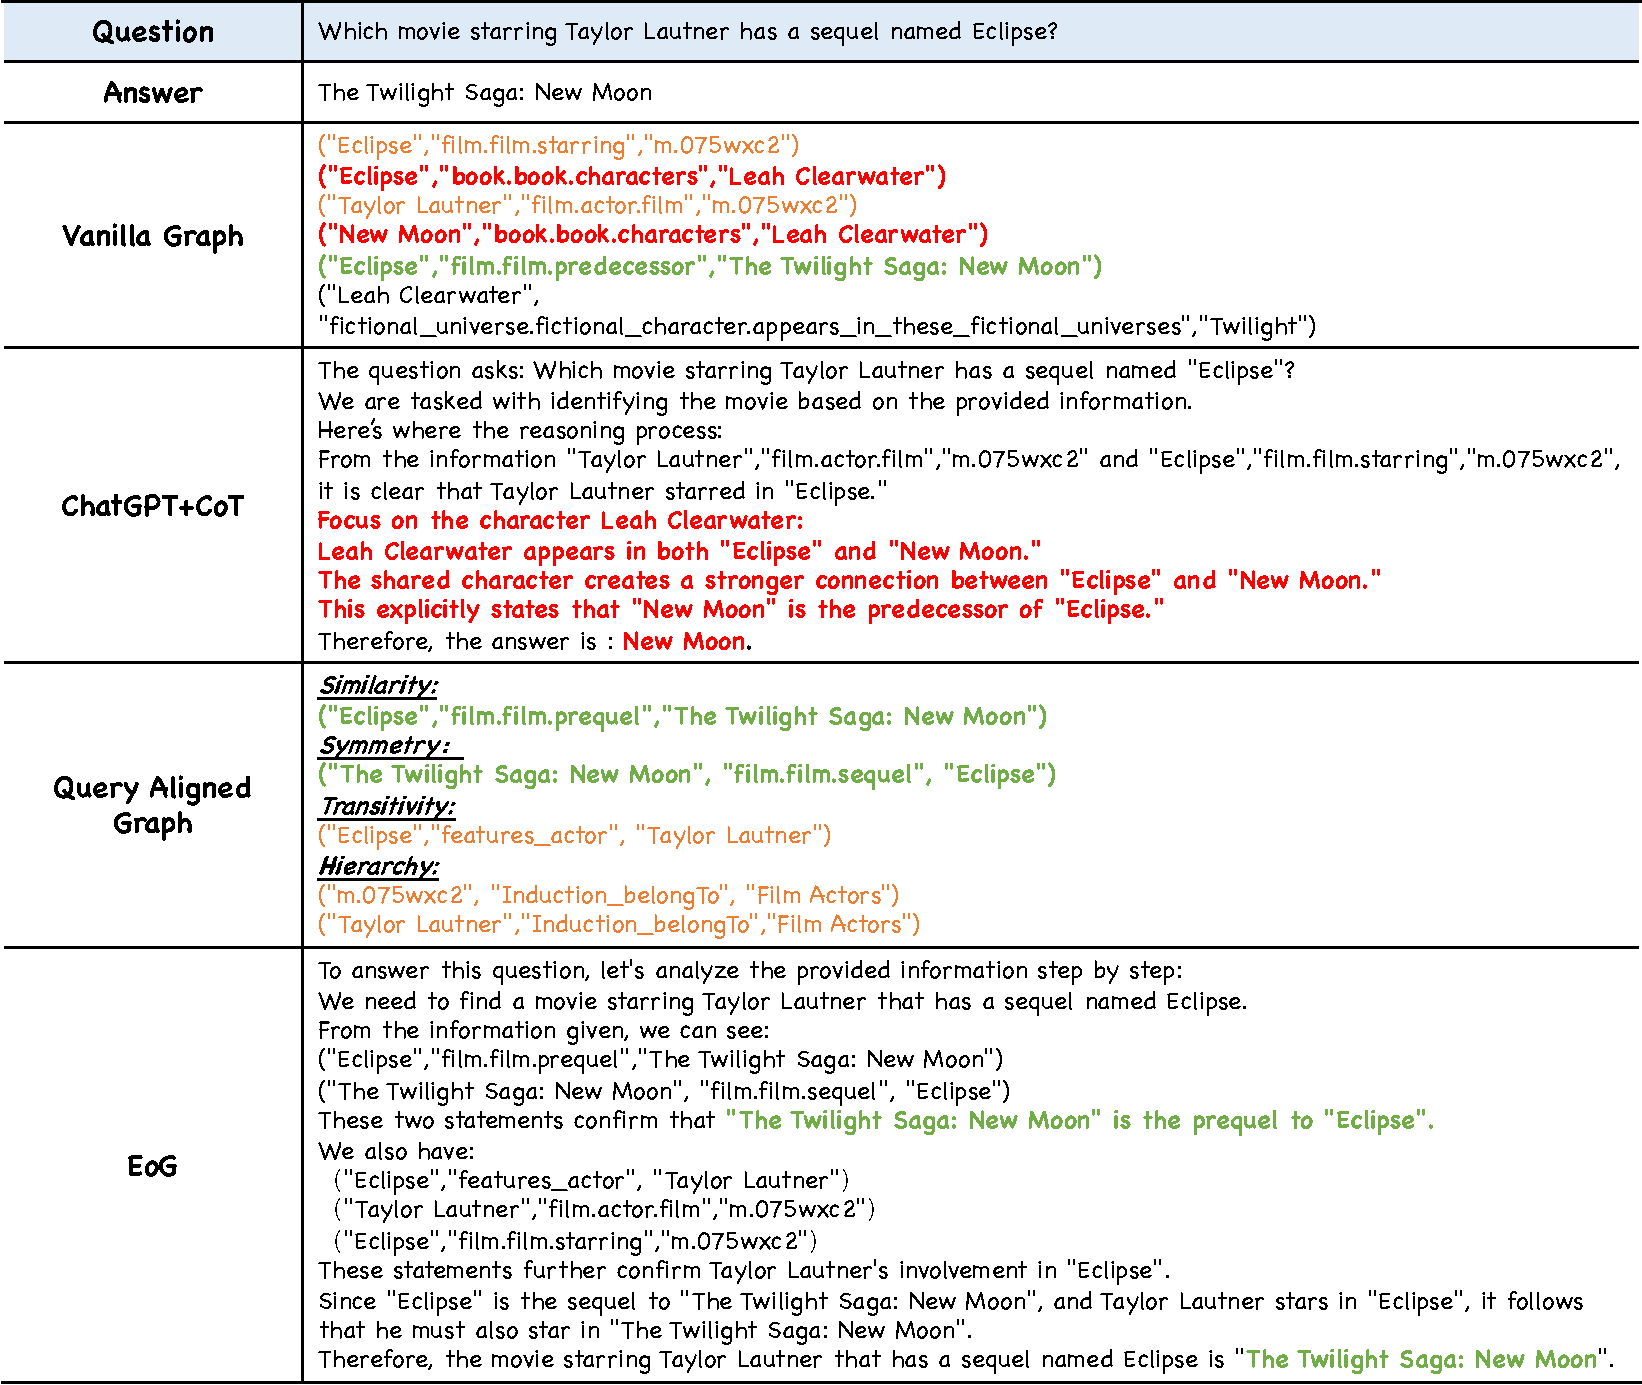
\includegraphics[width=\textwidth, keepaspectratio]{fig/case2.pdf}
    \caption{Case for EoG. \textbf{Green} highlights the correct answers or key triples, \textbf{Red} indicates misleading triples, and \textbf{Orange} represents triples relevant to the query.}
    \label{fig:case2}
\end{figure*}

In the second example, the vanilla KG contains ambiguous information: (\textit{Eclipse, film.film.starring, m.075wxc2}), and incorrect triples: (\textit{Eclipse, book.book.characters, Leah Clearwater}), (\textit{New Moon, book.book.characters, Leah Clearwater}). These lead ChatGPT to assume that \textit{Leah Clearwater’s} presence in both \textit{Eclipse} and \textit{New Moon} implies a chronological relationship, resulting in the wrong answer: \textit{New Moon}.
In contrast, EoG's query-aligned graph generates: (\textit{Eclipse}, \textit{film.film.prequel}, \textit{The Twilight Saga: New Moon}), which clarifies the prequel relationship between \textit{Eclipse} and the correct answer, \textit{The Twilight Saga: New Moon}. Additionally, the transitive triple: (\textit{Eclipse}, \textit{features\_actor}, \textit{Taylor Lautner}) helps LLMs verify the connection between \textit{Taylor Lautner} and \textit{Eclipse} from the query, leading to the correct reasoning and answer.

These examples demonstrate that EoG-generated query-aligned graphs not only bridge semantic gaps but also reduce reasoning complexity, enabling LLMs to perform more accurate and efficient reasoning.


\section{Impact of different base models and temperature parameters}
\label{plug-and-play-base-model}

% \begin{table}[]
% \resizebox{\linewidth}{!}{
% \begin{tabular}{l|ccccc}
% \toprule
% \multicolumn{1}{c|}{\multirow{2}{*}{Model}} & \multicolumn{2}{c}{CWQ} & \multicolumn{2}{c}{WebQSP} \\ 
% \multicolumn{1}{c|}{} & \textit{Hit@1} & \textit{F1} & \textit{Hit@1} & \textit{F1} \\ \midrule
% GPT-4o-mini & 70.8 & 65.0 & 85.0 & 74.1 \\
% {GPT-4o-mini}$^*$ & 70.9 & 65.1 & \textbf{85.1} & \textbf{74.7} \\
% GPT-4o-mini\textdagger  & 70.6 & 64.7 & 84.8 & 73.8 \\ \midrule
% GPT-3.5-turbo & 65.5 & 60.7 & 83.8 & 73.2 \\
% GPT-4o & \textbf{72.1} & \textbf{65.9} & 82.9 & 71.4 \\ \bottomrule
% \end{tabular}
% }
% \caption{Impact of different base models and temperature parameters. * indicates temperature is 0.5, while \textdagger \quad indicates temperature is 0.7.}
% \label{fig:Impact of different base models and temperature parameters}
% \end{table}


\begin{table}[]
\resizebox{\linewidth}{!}{
\begin{tabular}{lcccc}
\hline
\multicolumn{1}{c}{\multirow{2}{*}{Model}} & \multicolumn{2}{c}{CWQ} & \multicolumn{2}{c}{WebQSP} \\ 
\multicolumn{1}{c}{} & \textit{Hit@1} & \textit{F1} & \textit{Hit@1} & \textit{F1} \\ \hline
\multicolumn{5}{c}{\textit{Opensource  LLMs of EoG}} \\ \hline
Qwen-2-7b-instruct & 61.5 & 59.3 & 77.2 & 66.2 \\
LLaMA-3.1-8b-instruct & 70.9 & 64.5 & 81.6 & 69.9 \\ \hline
\multicolumn{5}{c}{\textit{Closed Source LLMs of EoG}} \\ \hline
GPT-4o-mini & 70.8 & 65.1 & 85.0 & 74.1 \\
{GPT-4o-mini}$^*$ & 70.9 & 65.1 & 85.1 & 74.8 \\
GPT-4o-mini\textdagger & 70.6 & 64.8 & 84.8 & 73.8 \\
GPT-3.5-turbo & 65.6 & 60.7 & 83.8 & 73.2 \\
GPT-4o & 72.1 & 66.0 & 82.9 & 71.4 \\
o3 & \textbf{77.6} & \textbf{71.0} & \textbf{85.9} & \textbf{75.1} \\ \hline
\end{tabular}
}
\caption{Impact of different base models and temperature parameters. * indicates temperature is 0.5, while \textdagger \quad indicates temperature is 0.7.}
\label{fig:Impact of different base models and temperature parameters}
\end{table}

As shown in Tab.~\ref{fig:Impact of different base models and temperature parameters}, we supplement our experiments by including the following additional LLM backbones: GPT-3.5-turbo, GPT4o, o3, LLaMA-3.1-8b-instruct, and Qwen2-7b-instruct. For the open-source small models LLaMA-3.1-8b-instruct and Qwen2-7b-instruct, we maintain the same training-free setup. This allows us to conduct a comprehensive evaluation across both open-source and closed-source LLMs, with varying model sizes and inference capabilities. The experimental results show that under our proposed framework, all LLM backbones demonstrate strong performance. Notably, even smaller parameter models like LLaMA and Qwen achieve performance comparable to advanced methods, despite using a training-free setup. Additionally, experiments with temperature settings of 0.2 (default), 0.5, and 0.7 showed differences below 1\%, verifying EoG's reproducibility and plug-and-play flexibility.


% Please add the following required packages to your document preamble:
% \usepackage{multirow}

\section{Performance on Different KGs}

We supplement our experiments with additional SOTA evaluations. Specifically, we conducted experiments on larger KGQA benchmarks, including GrailQA \cite{10.1145/3442381.3449992} (based on Freebase) and QALD10-en \cite{perevalov2022qald9plusmultilingualdatasetquestion} (on the larger knowledge graph Wikidata \cite{10.1145/2629489}). Combined with the original experimental results in Tab. \ref{main result}, our method demonstrates consistent superiority across KGQA benchmarks of varying scales, further validating its strong generalization ability. Specifically, as shown in Tab. \ref{table:grailqa}, on GrailQA, our method improves Hit@1 scores by 12.5\%, 6.8\%, 16.8\%, and 7.7\% compared to TIARA \cite{shu-etal-2022-tiara}, DECAF \cite{yu2023decafjointdecodinganswers}, ToG, and DoG, respectively, and outperforms TIARA on F1 score by 1.1\%. As shown in Tab. \ref{table:qald10-en}, on the QALD10-en dataset, our method achieves a 12.1\% improvement over ToG.

\begin{table}[]
\centering
\resizebox{0.5\linewidth}{!}{
\begin{tabular}{lcc}
\hline
\multicolumn{1}{c}{\multirow{2}{*}{Model}} & \multicolumn{2}{c}{GrailQA} \\
\multicolumn{1}{c}{} & \textit{Hits@1} & \textit{F1} \\ \hline
\multicolumn{3}{c}{\textit{LLMs Methods}} \\ \hline
IO & 29.4 & - \\
CoT & 28.1 & - \\ \hline
\multicolumn{3}{c}{\textit{LLMs+KG Methods}} \\ \hline
TIARA & 73.0 & 78.5 \\
DECAF & 78.7 & - \\
DoG & 68.7 & - \\
ToG & 77.8 & - \\
EoG & \textbf{85.5} & \textbf{79.6} \\ \hline
\end{tabular}
}
\caption{Performace comparision between advanced methods and EoG on GrailQA. Specifically, we followed ToG and randomly sampled 1000 examples from GrailQA for testing. Best results are in bold.}
\label{table:grailqa}
\end{table}

% Please add the following required packages to your document preamble:
% \usepackage{multirow}
\begin{table}[]
\centering
\resizebox{0.45\linewidth}{!}{
\begin{tabular}{lc}
\hline
\multicolumn{1}{c}{\multirow{2}{*}{Model}} & QALD10-en \\
\multicolumn{1}{c}{} & \textit{Hits@1} \\ \hline
\multicolumn{2}{c}{\textit{LLMs Methods}} \\ \hline
IO & 42.0 \\
CoT & 62.3 \\ \hline
\multicolumn{2}{c}{\textit{LLMs+KG Methods}} \\ \hline
ToG & 50.2 \\
EoG & \textbf{62.3} \\ \hline
\end{tabular}
}
\caption{Performace comparision between advanced methods and EoG on QALD10-en. Best results are in bold.}
\label{table:qald10-en}
\end{table}

\section{Elaboration of Focus-Aware Multi-Channel Pruning}
\label{elaboration-Focus-Aware Multi-Channel Pruning}
In this section, we will elaborate on the design rationale of Multi-Channel Pruning. Assuming the target answer triple for a query is ($e_1$, $r$, ?), where $e_1$ is the topic entity in the query, we describe three possible situations:
\begin{itemize}
\item \textbf{Situation 0}: The answer triple in the KG is ($e_1$, $r$, $e_2$).
\item \textbf{Situation 1}: The answer triple in the KG is ($e_1$, $r'$, $e_2$), where $r'$ is semantically similar to r but not strongly related.
\item \textbf{Situation 2}: The answer path involves two triples: ($e_1$, $r$, mid) and (mid, $r'$, $e_2$), where mid is an intermediatse entity, and $r'$ is semantically similar to $r$ but not strongly related.
\end{itemize}
Vanilla pruning effectively retrieves ($e_1$, $r$, $e_2$) in Situation 0. However, it often fails to retrieve ($e_1$, $r'$, $e_2$) in Situation 1 and (mid, $r'$, $e_2$) in Situation 2 because these triples are not semantically similar to the query ($e_1$, $r$, ?), resulting in lower similarity rankings. This failure to retrieve the correct triples leads to focus mismatch and often retrieves noise instead of answer triples.
To address these issues, our Three Masking channels are as follows:
\begin{itemize}
\item ($e_1$, $r$, MASK)

\item (MASK, $r$, $e_2$)

\item (MASK, $r$, MASK)
\end{itemize}
The ($e_1$, $r$, MASK) channel and (MASK, $r$, $e_2$) channel focus solely on the head or tail entity and the relation, thereby effectively retrieving triples like ($e_1$, $r'$, $e_2$) in Situation 1. The (MASK, $r$, MASK) channel focuses solely on the relation, thereby effectively retrieving triples like (mid, $r'$, $e_2$) in Situation 2. By combining the strengths of all three channels, the Three Masking mechanism can reliably retrieve the desired answer triples.

To better illustrate the contribution of each channel, we supplemented the paper with channel contribution experiments. We use the MRR (Mean Reciprocal Rank) metric to measure the ability of each channel to rank answer triples (i.e., the essential triples needed to answer the query). A higher MRR indicates that the answer triples are ranked higher within the channel and are more likely to be retrieved. We conducted these experiments on the WebQSP and CWQ datasets, as shown in Tab. \ref{table:three-channel-pruning}. Results show that a single channel's MRR score is similar to vanilla pruning, but combining three channels achieves the highest MRR, exceeding vanilla pruning by 0.002. This demonstrates that the Three Masking Pruning more effectively mitigates the focus mismatch.

\begin{table}[]
\centering
\resizebox{\linewidth}{!}{
\begin{tabular}{lcc}
\hline
\multicolumn{1}{l}{Pruning Method} & WebQSP & CWQ \\ \hline
Vanilla Pruning ($e_1$,$r$,$e_2$) & 0.0058 & 0.0049 \\
Channel ($e_1$,$r$,MASK) & 0.0056 & 0.0048 \\
Channel 2(MASK,$r$,$e_2$) & 0.0055 & 0.0051 \\
Channel 3 (MASK,$r$,MASK) & 0.0071 & 0.0059 \\
Three Channel Pruning (Combined) & 0.0078 & 0.0075 \\ \hline
\end{tabular}
}
\caption{MRR scores comparision between vanilla pruning and our Three Channel Pruning.}
\label{table:three-channel-pruning}
\end{table}

We demonstrate the contribution of each channel by calculating the proportion of its MRR score to the sum of MRR scores across all channels, as shown in Tab. \ref{table:channel-contrbution}. We found that the (MASK, $r$, MASK) channel contributes significantly more on both datasets than the other two channels, proving its effectiveness in addressing Situation 2.

\begin{table}[]
\centering
\resizebox{\linewidth}{!}{
\begin{tabular}{lccc}
\hline
\multicolumn{1}{l}{Dataset} & ($e_1$,$r$,MASK) & (MASK,$r$,$e_2$) & (MASK,$r$,MASK) \\ \hline
WebQSP & 30.72\% & 30.08\% & 39.18\% \\
CWQ & 30.48\% & 32.28\% & 37.22\% \\ \hline
\end{tabular}
}
\caption{Contribution of each channel.}
\label{table:channel-contrbution}
\end{table}

\section{Error Analysis}

We supplement our paper with an error analysis during the enrichment process. Specifically, we categorized errors during enrichment into three types:

\begin{itemize}
    \item \textbf{Identify Errors}: LLMs enrich triples that are unrelated to the query.

    \item \textbf{Structural Enrich Errors}: LLMs introduce incorrect or query-irrelevant relationships/paths during structural enrichment.

    \item \textbf{Feature Enrich Errors}: LLMs generate incorrect or query-irrelevant ontology during feature enrichment.
\end{itemize}

To analyze these errors, we randomly selected 100 samples from the WebQSP dataset and conducted a statistical evaluation, as shown in Tab. \ref{table:error-analysis-enrich}.

\begin{table}[]
\centering
\resizebox{\linewidth}{!}{
\begin{tabular}{ccc}
\hline
identify errors & structural enrich errors & feature enrich errors \\ \hline
8 & 1 & 2 \\ \hline
\end{tabular}
}
\caption{Error analysis during enrichment process.}
\label{table:error-analysis-enrich}
\end{table}

Our results indicate that identify errors are the primary cause of hallucinated knowledge during the enrichment process. This suggests that there is space for improvement in LLMs' ability to accurately identify query-relevant triples.

To demonstrate that our method effectively mitigates the hallucination problem of LLMs in KGQA, we performed an error analysis comparing our method with baseline methods. Following the error taxonomy from ToG, we categorized the errors: \textbf{1.Hallucination}; \textbf{2.Refuse Error}; \textbf{3.Format Error}. On the WebQSP dataset, we randomly selected 100 samples for statistical analysis, as shown in Tab. \ref{table:error-analysis-cmp}. The results show that our method halves hallucinations compared to standard prompts (IO) and chain of thought (CoT) while significantly reducing refuse errors by leveraging query-aligned KGs.

\begin{table}[]
\centering
\resizebox{\linewidth}{!}{
\begin{tabular}{lccc}
\hline
\multicolumn{1}{c}{Model} & halluciation & refuse error & format errors \\ \hline
IO & 23 & 16 & 13 \\
CoT & 20 & 35 & 13 \\
EoG & 11 & 1 & 11 \\ \hline
\end{tabular}
}
\caption{Error analysis comparison with baseline methods.}
\label{table:error-analysis-cmp}
\end{table}

\end{document}
